\documentclass{thesis}
\usepackage[utf8]{inputenc}
\usepackage[T5]{fontenc}
\usepackage{graphicx}
\usepackage{float}
\usepackage{mathptmx}
\usepackage{geometry}
\usepackage{xcolor}
\usepackage[fontsize=13pt]{scrextend}
\usepackage{indentfirst}
\usepackage{cite}
\usepackage{graphicx,subfigure}
\usepackage{amssymb,amsmath}
\usepackage{algorithm}
\usepackage{algorithmicx}
\usepackage{algpseudocode}
\usepackage{pifont}
\usepackage{float}
\usepackage[draft]{todonotes}
\usepackage{xargs}
\usepackage{comment}
\usepackage{color}
\usepackage{flushend}

%% --- Packages bổ sung cho nội dung thesis ---
\usepackage{booktabs}          % \toprule, \midrule, \bottomrule
\usepackage{threeparttable}    % \begin{tablenotes}
\usepackage{multirow}
\usepackage{makecell}
\usepackage{listings}          % code listing (C++, bash)
\usepackage{tikz}
\usetikzlibrary{shapes.geometric, arrows.meta, positioning, fit, calc}
\usepackage{pgfplots}
\pgfplotsset{compat=1.18}

\lstset{
  basicstyle=\ttfamily\small,
  breaklines=true,
  frame=single,
  numbers=left,
  numberstyle=\tiny\color{gray},
  keywordstyle=\color{blue!70!black},
  commentstyle=\color{green!50!black},
  stringstyle=\color{red!60!black},
  showstringspaces=false,
}

\newcommand{\eoproof}{\hfill $\square$}
\newtheorem{theorem}{\bf Theorem}[section]
\newtheorem{definition}{\bf Definition}[section]
\clearpage


%% START DOCUMENT
\begin{document}

%% ================================================================
%%  TRANG BÌA
%% ================================================================
\begin{center}
    \vspace{12pt}
        \textbf{\fontsize{15pt}{0pt} \selectfont{} ĐẠI HỌC BÁCH KHOA HÀ NỘI \\ \vspace{3pt} TRƯỜNG ĐIỆN - ĐIỆN TỬ}
    \vspace{0.5cm}

\begin{figure}[H]
    \centering
    
\includegraphics[width=2cm,height=3cm]{logoBK.png}
\end{figure}

\vspace{48pt}
        \fontsize{25pt}{0pt}\selectfont{} \textbf{ĐỒ ÁN TỐT NGHIỆP}
\vspace{24pt}

        \textbf{\fontsize{17pt}{0pt}\selectfont{} Hệ thống mã hoá video chuẩn H.264 ứng dụng thuật toán mã hoá hỗn loạn đa chiều triển khai trên FPGA}
    \vspace{18pt}

        \fontsize{14pt}{0pt}\selectfont{} \textbf{NGUYỄN Hoàng Minh}
    \vspace{3pt}

        \fontsize{14pt}{0pt}\selectfont{} minh.nh223724@sis.hust.edu.vn
    \vspace{12pt}

        \fontsize{14pt}{0pt}\selectfont{} \textbf{Ngành Kỹ thuật Điện tử Viễn thông}
\end{center}

\begin{table}[H]
    \centering
        \begin{tabular}{l l c}
            \textbf{Giảng viên hướng dẫn:}    &  TS. Tạ Thị Kim Huệ \vspace{6pt} &  \\
            &\vspace{3pt} & \fontsize{10pt}{0pt}\selectfont{} Chữ ký của GVHD \\
            \textbf{Khoa:} & Điện tử \vspace{3pt}\\
            \textbf{Trường:} & Điện - Điện tử
        \end{tabular}
\end{table}

\begin{center}
    \vspace{48pt}
    \fontsize{14pt}{0pt}\selectfont{} Hà Nội, 06/2026
\end{center}

\thispagestyle{empty}
    \newpage
        \clearpage
            \thispagestyle{empty}
                \cleardoublepage

%% ================================================================
%%  LỜI CAM ĐOAN
%% ================================================================
\section*{LỜI CAM ĐOAN}
    \thispagestyle{empty}
Em là Nguyễn Hoàng Minh, sinh viên lớp ET-TN K67. Em xin cam đoan nội dung trình bày trong đồ án ``Hệ thống mã hoá video chuẩn H.264 ứng dụng thuật toán mã hoá hỗn loạn đa chiều triển khai trên FPGA'' theo sự hướng dẫn của TS Tạ Thị Kim Huệ là kết quả trong quá trình nghiên cứu của em. Các kết quả đưa ra là trung thực và thực tế. Các thông tin, tài liệu tham khảo được trích dẫn đều tuân thủ các quy định về quyền sở hữu trí tuệ, các tài liệu được chú thích, liệt kê đầy đủ. Em xin chịu trách nhiệm với những nội dung được trình bày trong đồ án này.

\vspace{6pt}
    \hspace{7cm}Hà Nội, ngày 26 tháng 06 năm 2026

        \hspace{8.6cm} Sinh viên thực hiện

\vspace{2cm}
    \hspace{8.6cm}\textbf{Nguyễn Hoàng Minh}

\thispagestyle{empty}
    \newpage
        \clearpage
            \thispagestyle{empty}
                \cleardoublepage

%% ================================================================
%%  LỜI CẢM ƠN
%% ================================================================
\newpage
\section*{LỜI CẢM ƠN}
    \thispagestyle{empty}
Đầu tiên, em xin cảm ơn tiến sỹ Tạ Thị Kim Huệ, người đã tận tình hướng dẫn em trong suốt quá trình thực hiện đồ án này rất nhiều. Cảm ơn cô vì đã luôn đồng hành cùng em từ những năm tháng đầu tiên của đại học, khi em chỉ là cô sinh viên không biết gì về những kiến thức mật mã, bảo mật; đến ngày em có thể tham gia nghiên cứu khoa học, viết bài và đứng trình bày kết quả trên các hội nghị. Cảm ơn tất cả những thành viên trong lab đã luôn hỗ trợ, động viên em trong suốt gần 3 năm tham gia mặc dù em vẫn còn nhiều thiếu sót.

Em xin chân thành cảm ơn.

\newpage
    \thispagestyle{empty}
        \clearpage
            \thispagestyle{empty}
                \cleardoublepage

%% ================================================================
%%  TÓM TẮT
%% ================================================================
\section*{TÓM TẮT ĐỒ ÁN}
    \thispagestyle{empty}
Đồ án này nghiên cứu và triển khai hệ thống mã hoá chọn lọc các hệ số DC trong luồng bit H.264 mà không cần re-encode video. Phương pháp mã hoá chọn lọc chỉ mã hoá 25 bytes hệ số DC tại offset cố định trong mỗi NAL Unit VCL, cho phép làm suy giảm chất lượng hình ảnh đáng kể (PSNR $\approx$ 7--8 dB) với chi phí tính toán thấp hơn nhiều so với mã hoá toàn bộ bitstream.

Thuật toán lai ghép (hybrid) được đề xuất kết hợp ba tầng: sinh khóa dòng hỗn loạn PLCM (Piecewise Linear Chaotic Map) phụ thuộc chỉ số NALU, hoán vị Arnold 2D Cat Map, và cơ chế khuếch tán chuỗi XOR. Cơ chế khuếch tán chuỗi đảm bảo một bit thay đổi ở đầu vào lan truyền qua toàn bộ 25 bytes ciphertext, đạt NPCR $> 99.6\%$ (chuẩn Wu et al.\ 2011).

Thuật toán được so sánh với ba phương pháp cơ sở: AES-128-CTR, DES-OFB, và RC4, trên hai chiến lược (S1: Type 1 + Type 5; S2: chỉ Type 5). Kết quả thực nghiệm trên file H.264 thực tế (19.348 NALU, 219 MB) cho thấy thuật toán hybrid đạt chỉ số bảo mật tốt nhất (Entropy $\approx$ 8.0 bits/byte, SSIM DC $\approx$ 0), trong khi RC4 nhanh nhất (769 ns/NALU). Tính đúng đắn byte-exact được đảm bảo tuyệt đối (BER = 0, SHA-256 PASS) cho tất cả 8 tổ hợp.

\thispagestyle{empty}
    \cleardoublepage

%% ================================================================
%%  MỤC LỤC
%% ================================================================
\pagenumbering{roman}
\tableofcontents
    \thispagestyle{empty}
        \newpage
            \thispagestyle{empty}
                \cleardoublepage

%% DANH MỤC HÌNH VẼ
{\let\oldnumberline\numberline
    \renewcommand{\numberline}{Hình~\oldnumberline}
        \listoffigures}
            \phantomsection\addcontentsline{toc}{section}{\numberline{} DANH MỤC HÌNH VẼ}
\newpage

%% DANH MỤC BẢNG BIỂU
{\let\oldnumberline\numberline
    \renewcommand{\numberline}{Bảng~\oldnumberline}
        \listoftables}
            \phantomsection\addcontentsline{toc}{section}{\numberline{} DANH MỤC BẢNG BIỂU}
\newpage

%% ================================================================
%%  NỘI DUNG CÁC CHƯƠNG
%% ================================================================
\pagenumbering{arabic}

%% Chương 1: Mở đầu
\clearpage
\phantomsection
\section*{CHƯƠNG 1. MỞ ĐẦU}
\addcontentsline{toc}{section}{\numberline{}CHƯƠNG 1. MỞ ĐẦU}
\setcounter{section}{1}
\setcounter{subsection}{0}
\setcounter{figure}{0}
\setcounter{table}{0}
\setcounter{equation}{0}

\subsection{Bối cảnh và động lực}

\subsubsection{Sự bùng nổ của video trực tuyến}

Trong thập kỷ vừa qua, lưu lượng video trực tuyến (video streaming) đã tăng trưởng
với tốc độ chưa từng có. Theo các báo cáo thị trường, video hiện chiếm hơn 80\%
tổng lưu lượng Internet toàn cầu, và con số này dự báo sẽ vượt 90\% vào năm 2030.
Sự tăng trưởng này xuất phát từ nhiều xu hướng đồng thời: sự phổ biến của các
nền tảng phát trực tuyến theo yêu cầu (video-on-demand --- VOD) như YouTube, Netflix,
TikTok; sự mở rộng của hội nghị truyền hình (video conferencing) sau đại dịch;
sự phát triển của các hệ thống giám sát an ninh (CCTV, body cam); và sự ra đời
của các ứng dụng thực tế tăng cường (AR) và thực tế ảo (VR).

Trong bức tranh đó, chuẩn nén video H.264/AVC (ITU-T H.264 / ISO/IEC 14496-10)
\cite{itu_h264} giữ vị trí thống trị trong nhiều năm. Mặc dù các chuẩn mới hơn như
H.265/HEVC hay AV1 đang dần được triển khai, H.264 vẫn là lựa chọn mặc định
trên phần lớn thiết bị và nền tảng nhờ sự cân bằng xuất sắc giữa hiệu quả nén,
tốc độ mã hoá/giải mã, và tính tương thích phần cứng. Phần lớn camera giám sát,
thiết bị di động, và hệ thống phát sóng đều xuất ra video ở định dạng H.264.

\subsubsection{Yêu cầu bảo mật nội dung video}

Khi video trở thành phương tiện truyền tải thông tin quan trọng, nhu cầu bảo vệ
nội dung video khỏi truy cập trái phép ngày càng trở nên cấp thiết. Các tình huống
điển hình bao gồm:

\begin{itemize}
  \item \textbf{Bảo vệ bản quyền:} Nội dung giải trí có giá trị cao (phim, thể thao)
        cần được mã hoá để tránh xem lậu (piracy). Các hệ thống DRM (Digital Rights
        Management) như Widevine, FairPlay đều dựa trên mã hoá video stream.

  \item \textbf{Video giám sát an ninh:} Hình ảnh camera tại ngân hàng, sân bay,
        cơ quan chính phủ phải được bảo mật trong quá trình truyền qua mạng để
        tránh rò rỉ thông tin nhạy cảm hoặc bị giả mạo.

  \item \textbf{Hội nghị truyền hình y tế và pháp lý:} Các buổi tư vấn y tế từ xa,
        phiên toà trực tuyến yêu cầu mức độ bảo mật cao theo quy định pháp luật.

  \item \textbf{Truyền dữ liệu trên kênh không tin cậy:} Video truyền qua mạng
        không dây, mạng công cộng có nguy cơ bị nghe lén (eavesdropping)
        hoặc tấn công man-in-the-middle.
\end{itemize}

\subsubsection{Hạn chế của mã hoá toàn bộ luồng bit}

Giải pháp truyền thống là mã hoá toàn bộ luồng bit video bằng AES-128 hoặc AES-256
ở chế độ CBC/CTR. Cách tiếp cận này đảm bảo an toàn tuyệt đối nhưng có những
hạn chế thực tiễn quan trọng:

\begin{itemize}
  \item \textbf{Chi phí tính toán cao:} Video 4K 30fps có thể có bitrate 50--100 Mbps.
        Mã hoá AES toàn bộ bitstream đòi hỏi xử lý $6$--$12$ MB dữ liệu mỗi giây,
        ngốn đáng kể tài nguyên CPU trên thiết bị nhúng không có AES-NI hardware.

  \item \textbf{Độ trễ tăng:} Trong các ứng dụng thời gian thực (live streaming,
        video call), mỗi mili-giây trễ thêm đều ảnh hưởng đến trải nghiệm người dùng.
        Mã hoá toàn bộ có thể tăng độ trễ lên 10--30 ms trên thiết bị nhúng.

  \item \textbf{Không tương thích với codec pipeline:} Một số hệ thống cần
        transcode video ở phía server trong khi vẫn bảo mật nội dung (proxy encryption),
        điều này không khả thi khi toàn bộ payload bị mã hoá.
\end{itemize}

Mã hoá chọn lọc (selective encryption) \cite{cheng_selective} ra đời như một giải pháp
trung gian: chỉ mã hoá phần quan trọng nhất của video (perceptually significant
components), giảm chi phí tính toán mà vẫn đảm bảo mức độ bảo vệ chấp nhận được.

\subsection{Vấn đề nghiên cứu}

\subsubsection{Hệ số DC trong H.264 --- vùng nhạy cảm nhất}

Trong chuẩn H.264/AVC, mỗi khối ảnh (macroblock) được nén qua ba bước chính:
dự đoán nội (intra prediction), biến đổi cosine rời rạc (DCT), và lượng tử hoá
(quantization). Sau quá trình này, hệ số DC (coefficient ở tần số 0---0) của
biến đổi DCT là giá trị thể hiện mức cường độ trung bình của khối ảnh.
Hệ số DC quyết định độ sáng/tối cơ bản của vùng ảnh tương ứng.

Từ góc độ bảo mật tri giác (perceptual security), hệ số DC là mục tiêu lý tưởng
vì hai lý do:
\begin{enumerate}
  \item \textbf{Tác động thị giác lớn:} Nhiễu loạn hệ số DC gây ra distortion
        có thể nhìn thấy ngay cả ở bitrate cao. PSNR của video bị nhiễu loạn DC
        giảm xuống khoảng 7--8 dB, tương đương mức méo hình nghiêm trọng.
        Thử nghiệm của chúng tôi trên file output.h264 xác nhận điều này.

  \item \textbf{Chi phí thấp:} DC bytes chiếm 25 byte/NALU --- dưới 0.01\%
        kích thước bitstream trung bình. Mã hoá chúng tiêu tốn không đáng kể
        so với decode toàn bộ video.
\end{enumerate}

\subsubsection{Điểm yếu của các thuật toán mã hoá stream thông thường}

Khi áp dụng AES-CTR, DES-OFB, hoặc RC4 vào mã hoá chọn lọc DC, một vấn đề thiết
kế quan trọng thường bị bỏ qua: \textbf{keystream reuse}. Nếu cùng khóa K và cùng
IV/counter/seed được dùng cho mọi NALU, thì:

\begin{equation}
\text{Enc}(P_1, K) = P_1 \oplus ks \quad\text{và}\quad \text{Enc}(P_2, K) = P_2 \oplus ks
\end{equation}

Nếu kẻ tấn công biết $P_1$ (DC bytes của một NALU thông qua phân tích thống kê),
hắn có thể tính $ks = \text{Enc}(P_1, K) \oplus P_1$, từ đó giải mã mọi NALU khác.

Vấn đề thứ hai là thiếu \textbf{diffusion}: nếu 1 bit của plaintext thay đổi,
chỉ 1 bit ciphertext thay đổi theo (không có hiệu ứng lan truyền). Điều này dẫn
đến NPCR (Number of Pixels Change Rate) thấp --- chỉ $\approx 4\%$ (1/25 bytes),
trong khi mã hoá mạnh cần NPCR $> 99.6\%$.

\subsubsection{Khoảng trống nghiên cứu}

Qua khảo sát các công trình liên quan (phần~\ref{subsec:related_work}), chúng tôi
nhận thấy phần lớn nghiên cứu mã hoá chọn lọc H.264 tập trung vào:
(a) lựa chọn vùng mã hoá (entropy coding, motion vectors, DC/AC),
(b) duy trì tính stream-compliant,
nhưng ít chú ý đến \textbf{per-NALU keystream variation} và \textbf{intra-NALU diffusion}
--- hai tính chất cần thiết để đảm bảo plaintext sensitivity (NPCR/UACI).

Nghiên cứu này lấp đầy khoảng trống đó bằng cách đề xuất thuật toán hybrid
kết hợp ánh xạ hỗn độn (PLCM) tạo keystream khác mỗi NALU, hoán vị Arnold,
và cơ chế khuếch tán chuỗi (chained diffusion feedback).

\subsection{Công trình liên quan}
\label{subsec:related_work}

\subsubsection{Mã hoá chọn lọc video H.264}

Cheng và cộng sự \cite{cheng_selective} đề xuất phân loại mã hoá chọn lọc
thành 3 cấp độ: header encryption, DC coefficient encryption, và motion vector
encryption. Nghiên cứu chứng minh rằng chỉ cần mã hoá DC là đủ để làm mờ nội dung
với chi phí dưới 5\% tổng chi phí mã hoá.

Shahid và cộng sự \cite{shahid_selective} nghiên cứu mã hoá chọn lọc cho
H.264 với yêu cầu duy trì định dạng (format compliance) --- video sau mã hoá
vẫn có thể được xử lý bởi các thiết bị H.264 tiêu chuẩn. Đây là ràng buộc
chặt hơn so với cách tiếp cận của chúng tôi.

\subsubsection{Mã hoá video dựa trên lý thuyết hỗn độn}

Chen và cộng sự \cite{chen_chaos_video} đề xuất sử dụng kết hợp logistic map
và Arnold Cat Map cho mã hoá toàn bộ frame video. Nghiên cứu chứng minh rằng
hệ thống hỗn độn kết hợp đạt NPCR $> 99.6\%$ và Entropy $\approx 8.0$.
Tuy nhiên, nghiên cứu đó áp dụng cho ảnh tĩnh, không tối ưu cho bitstream H.264.

Nghiên cứu của chúng tôi kế thừa ý tưởng kết hợp PLCM và Arnold từ \cite{chen_chaos_video}
nhưng thích nghi cho cấu trúc NALU của H.264 với cơ chế per-NALU nalu\_index
--- điểm khác biệt then chốt.

\subsubsection{NPCR/UACI như chỉ số đánh giá}

Wu và cộng sự \cite{wu_npcr} hệ thống hoá các chỉ số NPCR và UACI, xác lập
ngưỡng lý thuyết cho mã hoá tốt: NPCR $> 99.6\%$ và UACI $\approx 33.46\%$.
Đây là framework đánh giá được chúng tôi áp dụng trực tiếp.

\subsection{Mục tiêu nghiên cứu}

Nghiên cứu này nhằm đạt các mục tiêu cụ thể sau:

\begin{enumerate}
  \item \textbf{Đề xuất thuật toán hybrid:} Thiết kế và cài đặt thuật toán
        mã hoá chọn lọc DC H.264 kết hợp PLCM, Arnold 2D Cat Map, và
        cơ chế khuếch tán chuỗi (chained diffusion feedback), đảm bảo
        per-NALU keystream variation.

  \item \textbf{So sánh hệ thống:} Cài đặt ba thuật toán so sánh (AES-128-CTR,
        DES-OFB, RC4) trong cùng pipeline, đánh giá trên các chỉ số đồng nhất:
        bảo mật (NPCR, UACI, Entropy, SSIM, TSSIM), hiệu năng (ns/NALU), và
        tính đúng đắn (BER, SHA-256).

  \item \textbf{Phân tích hai chiến lược:} Đánh giá S1 (toàn bộ VCL) và S2
        (chỉ I-frame) về hiệu năng và bảo mật, làm rõ trade-off giữa phạm vi
        mã hoá và chi phí tính toán.

  \item \textbf{Thiết kế kiến trúc mở rộng:} Xây dựng IEncryption interface
        (C++) cho phép tích hợp thuật toán mới mà không thay đổi pipeline
        --- hướng tới triển khai FPGA trong tương lai.
\end{enumerate}

\subsection{Phạm vi nghiên cứu}

Để đảm bảo tính tập trung và khả năng tái hiện, nghiên cứu này được giới hạn
trong phạm vi sau:

\begin{itemize}
  \item \textbf{Định dạng video:} H.264 raw bitstream (Annex B format). Không
        hỗ trợ container (MP4, MKV) hoặc các chuẩn khác (H.265, AV1, VP9).

  \item \textbf{Vùng mã hoá:} Chỉ DC bytes tại offset 19, kích thước 25 bytes
        trong mỗi NALU VCL. Không mã hoá SPS, PPS, SEI, motion vectors,
        AC coefficients, hay Cabac data.

  \item \textbf{Dataset:} Một file H.264 duy nhất (\texttt{output.h264}),
        kích thước 219 MB, 19.348 NALU tổng cộng. Đây là hạn chế được thừa
        nhận (xem Chương 7).

  \item \textbf{Môi trường thực thi:} Linux Ubuntu 22.04 (x86-64), GCC 11,
        Python 3.12. Không bao gồm FPGA triển khai phần cứng (là hướng phát triển).

  \item \textbf{Mô hình đe doạ:} Nghiên cứu tập trung vào \emph{perceptual security}
        (làm mờ nội dung thị giác) và \emph{plaintext sensitivity}.
        Không phân tích IND-CCA, side-channel attacks, hay key management.
\end{itemize}

\subsection{Đóng góp của nghiên cứu}

Các đóng góp chính của nghiên cứu này bao gồm:

\begin{enumerate}
  \item \textbf{Thuật toán hybrid mới:} Đề xuất kết hợp PLCM + Arnold 2D + XOR
        + chained diffusion vào mã hoá DC H.264, đạt NPCR $> 99.69\%$ (S2)
        và Entropy $\approx 8.0$ --- vượt ngưỡng tiêu chuẩn.

  \item \textbf{Phân tích pipeline paradox:} Lần đầu tiên mô tả và giải thích
        hiện tượng ``pipeline convergence'' trong S2 --- khi DC $< 1\%$
        tổng thời gian pipeline, tốc độ thuật toán không ảnh hưởng đến thời gian tổng.

  \item \textbf{Bộ dữ liệu thực nghiệm đầy đủ:} Cung cấp kết quả 12 chỉ số
        cho 8 tổ hợp (4 thuật toán $\times$ 2 chiến lược) trên cùng một file
        H.264, cho phép so sánh công bằng (apples-to-apples comparison).

  \item \textbf{Kiến trúc phần mềm mở rộng:} IEncryption interface cho phép
        thêm thuật toán mới với 0 thay đổi pipeline --- nền tảng cho triển khai
        FPGA và nghiên cứu tiếp theo.
\end{enumerate}

\subsection{Cấu trúc báo cáo}

Phần còn lại của báo cáo được tổ chức như sau:

\begin{itemize}
  \item \textbf{Chương 2 --- Cơ sở lý thuyết:} Trình bày nền tảng kiến thức về
        chuẩn H.264/AVC (cấu trúc NALU, hệ số DC, cơ chế nén intra), các nguyên
        lý mật mã hỗn độn (PLCM, Arnold Cat Map), các thuật toán mã hoá cổ điển
        (AES, DES, RC4), và framework đánh giá (NPCR, UACI, Entropy, SSIM, BER).

  \item \textbf{Chương 3 --- Phương pháp đề xuất:} Mô tả chi tiết thiết kế
        thuật toán hybrid, bao gồm PLCM keystream generation, Arnold permutation,
        XOR và chained diffusion, giải mã, phân tích bảo mật và keyspace.

  \item \textbf{Chương 4 --- Các thuật toán so sánh:} Phân tích AES-128-CTR,
        DES-OFB, RC4 từ góc độ điểm yếu bảo mật trong ngữ cảnh mã hoá chọn lọc,
        giải thích lý do NPCR/UACI không áp dụng cho các thuật toán này.

  \item \textbf{Chương 5 --- Thiết lập thực nghiệm:} Mô tả môi trường phần
        cứng/phần mềm, dataset, pipeline C++ end-to-end, và quy trình đo metrics.

  \item \textbf{Chương 6 --- Kết quả và thảo luận:} Phân tích toàn bộ kết quả
        thực nghiệm về tính đúng đắn, hiệu năng, và bảo mật cho tất cả
        8 tổ hợp thuật toán-chiến lược.

  \item \textbf{Chương 7 --- Kết luận:} Tổng kết đóng góp, nhận xét hạn chế
        của nghiên cứu, và đề xuất hướng phát triển trong tương lai.
\end{itemize}

%% Chương 2: Cơ sở lý thuyết
\clearpage
\phantomsection
\section*{CHƯƠNG 2. CƠ SỞ LÝ THUYẾT}
\addcontentsline{toc}{section}{\numberline{}CHƯƠNG 2. CƠ SỞ LÝ THUYẾT}
\setcounter{section}{2}
\setcounter{subsection}{0}
\setcounter{figure}{0}
\setcounter{table}{0}
\setcounter{equation}{0}

\subsection{Chuẩn H.264/AVC}

\subsubsection{Lịch sử và vị trí của H.264}

H.264/AVC (Advanced Video Coding) là chuẩn nén video được phát triển chung bởi
ITU-T Video Coding Experts Group (VCEG) và ISO/IEC Moving Picture Experts Group (MPEG),
được công bố lần đầu năm 2003 và liên tục cập nhật đến nay \cite{itu_h264}.
Chuẩn này có tên gọi song song là H.264 (trong hệ thống ITU-T) và MPEG-4 AVC
(trong hệ thống ISO/IEC 14496-10).

So với các chuẩn tiền nhiệm như H.263 hay MPEG-2, H.264 đạt mức nén gấp 2 lần
tại cùng chất lượng hình ảnh. Điều này đạt được thông qua nhiều kỹ thuật tiên tiến
như dự đoán chuyển động đa tham chiếu (multi-reference motion prediction), biến đổi
integer DCT 4$\times$4, mã hoá entropy CABAC (Context-Adaptive Binary Arithmetic Coding),
và deblocking filter. Sự kết hợp giữa chất lượng nén cao và tính tương thích phần cứng
rộng làm cho H.264 trở thành chuẩn video phổ biến nhất trong suốt hơn hai thập kỷ.

\subsubsection{Kiến trúc phân lớp của H.264}

Chuẩn H.264 được thiết kế theo kiến trúc hai lớp tách biệt:

\begin{itemize}
  \item \textbf{VCL (Video Coding Layer):} Lớp mã hoá video thuần túy, chịu trách
        nhiệm nén dữ liệu ảnh. VCL xử lý các slice (đơn vị mã hoá độc lập),
        macroblock (khối ảnh 16$\times$16 pixel), và các phép biến đổi toán học.

  \item \textbf{NAL (Network Abstraction Layer):} Lớp trừu tượng mạng, đóng gói
        dữ liệu VCL thành các đơn vị NALU (NAL Unit) phù hợp với truyền tải
        qua các giao thức mạng khác nhau (RTP, HTTP, v.v.) hoặc lưu trữ.
\end{itemize}

Sự tách biệt này cho phép cùng một chuẩn nén hoạt động trên nhiều môi trường
truyền tải khác nhau mà không cần thay đổi phần mã hoá video cốt lõi.

\subsubsection{Cấu trúc NAL Unit (NALU)}

Mỗi NAL Unit là đơn vị cơ bản của luồng bit H.264. Trong định dạng Annex B
(byte stream format --- định dạng được sử dụng trong nghiên cứu này), mỗi NALU
được ngăn cách bởi start code:

\begin{itemize}
  \item Start code 4 bytes: \texttt{0x00 0x00 0x00 0x01}
  \item Hoặc start code 3 bytes: \texttt{0x00 0x00 0x01} (cho các NALU không phải đầu tiên trong access unit)
\end{itemize}

Sau start code là payload của NALU, bắt đầu bằng \textbf{NAL header} (1 byte) với cấu trúc:

\begin{table}[ht]
\centering
\caption{Cấu trúc byte NAL header (1 byte)}
\label{tab:nal_header}
\begin{tabular}{cccl}
\toprule
Bit & Tên trường & Kích thước & Ý nghĩa \\
\midrule
7   & forbidden\_zero\_bit  & 1 bit  & Luôn = 0 (kiểm tra lỗi) \\
5-6 & nal\_ref\_idc         & 2 bits & Mức độ tham chiếu (0: không tham chiếu) \\
0-4 & nal\_unit\_type       & 5 bits & Loại NALU (xem Bảng~\ref{tab:nal_types}) \\
\bottomrule
\end{tabular}
\end{table}

\subsubsection{Phân loại NAL Unit}

Trường \texttt{nal\_unit\_type} (5 bit thấp của NAL header) xác định loại dữ liệu
trong NALU:

\begin{table}[ht]
\centering
\caption{Các loại NAL Unit quan trọng trong H.264}
\label{tab:nal_types}
\begin{tabular}{cll}
\toprule
\texttt{nal\_unit\_type} & Tên & Ý nghĩa \\
\midrule
1 & Coded slice (non-IDR) & P-frame (predictive) hoặc B-frame (bi-predictive) \\
2 & Coded slice data partition A & Phân vùng dữ liệu (ít phổ biến) \\
5 & IDR (Instantaneous Decoding Refresh) slice & I-frame (Intra-coded) --- keyframe \\
6 & SEI                   & Supplemental Enhancement Information \\
7 & SPS                   & Sequence Parameter Set (thông số chung) \\
8 & PPS                   & Picture Parameter Set (thông số ảnh) \\
9 & Access Unit Delimiter & Dấu phân cách access unit \\
\bottomrule
\end{tabular}
\end{table}

\textbf{Phân loại trong nghiên cứu:}
\begin{itemize}
  \item \textbf{VCL NALU (Video Coding Layer):} Type 1 và Type 5 chứa dữ liệu ảnh
        thực sự và là đối tượng mã hoá trong nghiên cứu này.
  \item \textbf{Non-VCL NALU:} Type 7 (SPS), Type 8 (PPS), Type 6 (SEI) chứa
        thông số cấu hình và metadata --- \textbf{không bị mã hoá}.
\end{itemize}

Trong file thực nghiệm \texttt{output.h264}, phân phối NALU như sau:
Type 5 (IDR/I-frame): 155 NALU; Type 1 (P/B-frame): 18.882 NALU; các loại khác: 311 NALU.
Chiến lược S1 mã hoá 19.037 VCL NALU (Type 1 + Type 5, bỏ qua 311 non-VCL),
S2 chỉ mã hoá 155 NALU Type 5.

\subsubsection{Intra Prediction và hệ số DC}

Để hiểu tầm quan trọng của hệ số DC, cần nắm cơ chế dự đoán intra của H.264.
Với I-frame (IDR slice, Type 5), mọi macroblock được mã hoá bằng \textbf{intra prediction}
--- dự đoán khối ảnh từ các khối đã được mã hoá trong cùng frame, không tham chiếu
frame khác. Quá trình xử lý một macroblock luma (16$\times$16 pixel) diễn ra như sau:

\begin{enumerate}
  \item \textbf{Intra prediction:} Dự đoán giá trị pixel từ các pixel lân cận đã biết.
        H.264 hỗ trợ 13 chế độ dự đoán intra 4$\times$4 và 4 chế độ 16$\times$16.
        Kết quả là \emph{residual} (sai lệch giữa thực tế và dự đoán).

  \item \textbf{Biến đổi integer DCT:} Residual $R$ (4$\times$4 hoặc 8$\times$8) được
        biến đổi bằng integer approximation của DCT:
        \begin{equation}
        Y = H \cdot R \cdot H^T
        \end{equation}
        trong đó $H$ là ma trận biến đổi integer DCT. Kết quả $Y$ có 16 hệ số,
        trong đó \textbf{hệ số DC là $Y[0,0]$} --- hệ số tần số thấp nhất,
        biểu diễn giá trị trung bình của khối residual.

  \item \textbf{Lượng tử hoá:} Các hệ số được lượng tử hoá theo QP (quantization parameter).
        Hệ số DC thường có weight lượng tử hoá khác với AC để bảo toàn chất lượng.

  \item \textbf{Mã hoá entropy:} Các hệ số sau lượng tử hoá được mã hoá bằng CAVLC
        hoặc CABAC và ghép vào bitstream.
\end{enumerate}

\subsubsection{Vị trí hệ số DC trong luồng bit NALU}

Qua phân tích bitstream bằng công cụ \texttt{h264\_analyze} \cite{h264bitstream},
chúng tôi xác định rằng đối với file \texttt{output.h264} (H.264 Baseline Profile),
các hệ số DC của slice header chiếm vùng bytes từ offset 19 đến 43 trong payload
NALU VCL (sau start code):

\begin{itemize}
  \item \texttt{DC\_OFFSET = 19}: Offset tính từ đầu payload NALU (sau start code).
  \item \texttt{DC\_SIZE = 25}: Kích thước vùng DC, 25 bytes.
  \item Vị trí tuyệt đối: \texttt{nal\_pos + 19} đến \texttt{nal\_pos + 43}
        (với \texttt{nal\_pos} là vị trí byte đầu của payload NALU trong file).
\end{itemize}

\begin{figure}[ht]
\centering
%% TikZ: DC offset diagram — byte layout trong NALU VCL
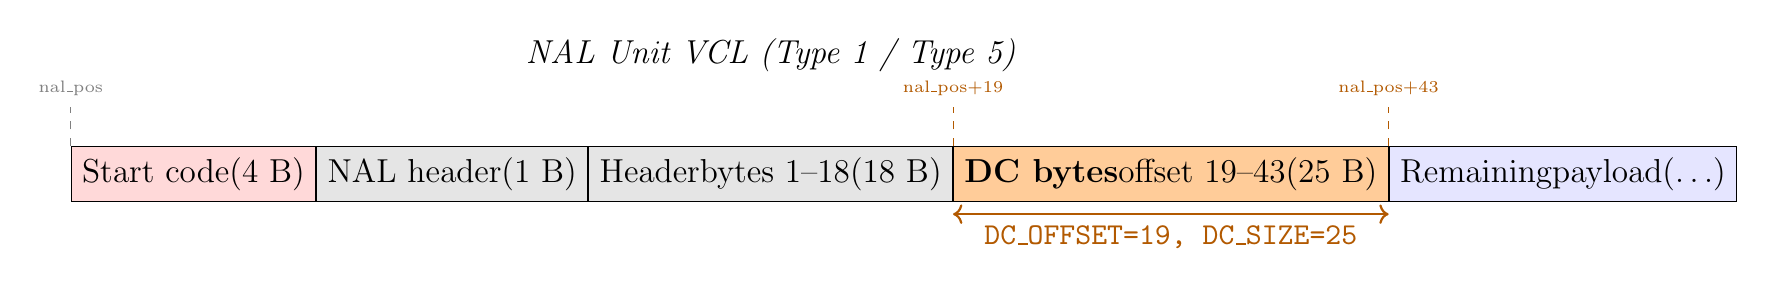
\begin{tikzpicture}[
  box/.style={draw, minimum height=0.7cm, font=\small},
  header/.style={box, fill=gray!20, minimum width=1.8cm},
  dc/.style={box, fill=orange!40, minimum width=3.5cm},
  rest/.style={box, fill=blue!10, minimum width=2.5cm},
  startcode/.style={box, fill=red!15, minimum width=1.6cm},
]

%% Row 1: byte layout
\node[startcode] (sc) at (0,0) {Start code\\(4 B)};
\node[header, right=0pt of sc] (nh) {NAL header\\(1 B)};
\node[header, right=0pt of nh] (hdr) {Header\\bytes 1–18\\(18 B)};
\node[dc, right=0pt of hdr] (dc) {\textbf{DC bytes}\\offset 19–43\\(25 B)};
\node[rest, right=0pt of dc] (rest) {Remaining\\payload\\($\ldots$)};

%% Annotations below
\draw[<->, thick, orange!70!black]
  ([yshift=-0.15cm]dc.south west) -- ([yshift=-0.15cm]dc.south east)
  node[midway, below, font=\footnotesize] {\texttt{DC\_OFFSET=19, DC\_SIZE=25}};

\draw[dashed, gray]
  (sc.north west) -- ++(0, 0.5) node[above, font=\tiny] {nal\_pos};
\draw[dashed, orange!70!black]
  (dc.north west) -- ++(0, 0.5) node[above, font=\tiny] {nal\_pos+19};
\draw[dashed, orange!70!black]
  (dc.north east) -- ++(0, 0.5) node[above, font=\tiny] {nal\_pos+43};

%% Label
\node[above=0.8cm of hdr, font=\small\itshape] {NAL Unit VCL (Type 1 / Type 5)};

\end{tikzpicture}

\caption{Bố cục byte trong NALU VCL: vùng DC (bytes 19--43) được tô màu cam;
         bytes 0--18 là header không mã hoá}
\label{fig:dc_offset}
\end{figure}

\textbf{Lưu ý quan trọng:} DC\_OFFSET = 19 được xác định bằng phân tích thực nghiệm
trên file cụ thể này (H.264 Baseline Profile). Với các profile khác (Main, High),
vị trí này có thể thay đổi --- đây là hạn chế được thảo luận trong Chương 7.

Các bytes 0--18 (header NALU) chứa thông tin slice như: frame number, picture order
count, reference frame index --- không được mã hoá để đảm bảo khả năng decode
frame (với error concealment) ngay cả khi DC bị mã hoá.

\begin{figure}[ht]
\centering
%% TikZ: H.264 NALU structure — bitsteram level
\begin{tikzpicture}[
  box/.style={draw, minimum height=0.75cm, text centered, font=\small},
  stream/.style={box, fill=gray!10, minimum width=1.2cm},
  nal/.style={box, fill=blue!12},
  vcl/.style={box, fill=green!15},
  nonvcl/.style={box, fill=yellow!20},
  arrow/.style={->, >=stealth},
]

%% Bitstream row
\node[stream, minimum width=0.8cm] (s0) at (0,0) {\ldots};
\node[nal, right=0pt of s0, minimum width=1.4cm] (sc1) {SC\\(4B)};
\node[nal, right=0pt of sc1, minimum width=0.8cm] (t7) {SPS\\T=7};
\node[nal, right=0pt of t7, minimum width=1.4cm] (sc2) {SC\\(4B)};
\node[nal, right=0pt of sc2, minimum width=0.8cm] (t8) {PPS\\T=8};
\node[nal, right=0pt of t8, minimum width=1.4cm] (sc3) {SC\\(4B)};
\node[vcl, right=0pt of sc3, minimum width=1.2cm] (t5) {IDR\\T=5};
\node[nal, right=0pt of t5, minimum width=1.4cm] (sc4) {SC\\(4B)};
\node[vcl, right=0pt of sc4, minimum width=1.2cm] (t1a) {P\\T=1};
\node[nal, right=0pt of t1a, minimum width=1.4cm] (sc5) {SC\\(4B)};
\node[vcl, right=0pt of sc5, minimum width=1.2cm] (t1b) {P\\T=1};
\node[stream, right=0pt of t1b, minimum width=0.8cm] (s1) {\ldots};

%% Zoom in to IDR NALU
\node[vcl, below=1.8cm of t5, minimum width=1.2cm] (idt) {IDR (T=5)};
\node[box, right=0pt of idt, fill=gray!20, minimum width=1.4cm] (hdr18) {Header\\1–18};
\node[box, right=0pt of hdr18, fill=orange!40, minimum width=2.0cm] (dc25) {\textbf{DC}\\25 bytes};
\node[box, right=0pt of dc25, fill=blue!10, minimum width=1.6cm] (rem) {Remain\\payload};

%% Arrow from T5 down
\draw[arrow, dashed] (t5.south) -- (idt.north);

%% DC annotation
\draw[<->, orange!80!black, thick]
  ([yshift=-0.15cm]dc25.south west) -- ([yshift=-0.15cm]dc25.south east)
  node[midway, below, font=\footnotesize] {offset 19..43};

%% Legend
\node[vcl, minimum width=0.6cm, minimum height=0.4cm] (leg1) at (0,-3.4) {};
\node[right=2pt of leg1, font=\footnotesize] {VCL (Type 1, 5) — được mã hoá};
\node[nonvcl, minimum width=0.6cm, minimum height=0.4cm, right=2.8cm of leg1] (leg2) {};
\node[right=2pt of leg2, font=\footnotesize] {Non-VCL (SPS, PPS) — không mã hoá};

\end{tikzpicture}

\caption{Cấu trúc luồng bit H.264: SPS, PPS, IDR (Type 5) và P-frames (Type 1);
         zoom vào IDR NALU cho thấy vùng DC 25 bytes}
\label{fig:nalu_structure}
\end{figure}

\subsection{Mã hoá chọn lọc (Selective Encryption)}

\subsubsection{Nguyên lý và phân loại}

Mã hoá chọn lọc \cite{cheng_selective} là cách tiếp cận mã hoá dựa trên tính
quan trọng tri giác (perceptual importance) của các thành phần video. Thay vì
mã hoá toàn bộ bitstream (chi phí cao), chỉ mã hoá phần tối thiểu đủ để:
\begin{enumerate}
  \item Làm mờ nội dung với người xem không có khóa (không thể hiểu nội dung).
  \item Duy trì khả năng truyền tải (bitstream có thể được parse/route mà không cần decrypt).
  \item Giảm chi phí tính toán xuống phần nhỏ so với full encryption.
\end{enumerate}

Các mức độ mã hoá chọn lọc từ ít đến nhiều:
\begin{itemize}
  \item \textbf{Header-only:} Chỉ mã hoá SPS/PPS --- file không decode được nhưng
        thiếu an toàn nếu attacker đoán được header.
  \item \textbf{DC-only (cách tiếp cận của chúng tôi):} Mã hoá hệ số DC --- balance
        tốt giữa chi phí và hiệu quả bảo vệ.
  \item \textbf{DC+Motion Vector:} Kết hợp DC và motion vectors để bảo vệ tốt hơn
        cho P/B-frames.
  \item \textbf{DC+AC low frequency:} Mã hoá DC và một số AC coefficients tần số thấp
        --- chi phí tăng nhưng bảo vệ mạnh hơn.
\end{itemize}

\subsubsection{Hai chiến lược S1 và S2}

Trong nghiên cứu này, chúng tôi so sánh hai chiến lược mã hoá DC:

\textbf{S1 --- Mã hoá toàn bộ VCL:}
Mã hoá DC của tất cả NALU có Type 1 (P/B-frame) và Type 5 (I-frame).
Với file test: 19.037 NALU được mã hoá / 19.348 tổng = 98.4\% NALU.
S1 bảo vệ mạnh nhất vì cả I-frame lẫn P/B-frames đều bị nhiễu loạn.

\textbf{S2 --- Chỉ mã hoá I-frame:}
Chỉ mã hoá DC của NALU Type 5 (IDR slice / I-frame).
Với file test: 155 NALU được mã hoá / 19.348 tổng = 0.8\% NALU.
S2 hy sinh bảo vệ P/B-frames để đổi lấy chi phí tính toán thấp hơn 120 lần.

\textbf{Lý do I-frame quan trọng hơn:} I-frame là keyframe độc lập --- toàn bộ
frame được mã hoá intra, không tham chiếu frame khác. Khi I-frame bị nhiễu loạn,
lỗi có thể lan truyền sang P/B-frames phụ thuộc vào nó. Tuy nhiên, trong thực tế,
H.264 có cơ chế error concealment nên P/B-frames vẫn hiển thị được (có méo hình).

\subsection{Lý thuyết hỗn độn (Chaos Theory) trong mật mã học}

\subsubsection{Tính chất của hệ hỗn độn}

Các hệ hỗn độn (chaotic systems) có ba tính chất cốt lõi làm cho chúng phù hợp
cho mật mã học \cite{chen_chaos_video}:

\begin{enumerate}
  \item \textbf{Nhạy cảm với điều kiện đầu (Sensitivity to Initial Conditions):}
        Hai quỹ đạo bắt đầu gần nhau sẽ phân kỳ theo hàm mũ theo thời gian.
        Được định lượng bởi \textbf{Lyapunov exponent} $\lambda > 0$: hai điểm
        ban đầu cách nhau $\delta_0$ sẽ cách nhau $\delta_0 e^{\lambda t}$ sau
        thời gian $t$. Với mật mã: thay đổi 1 bit khóa dẫn đến keystream
        hoàn toàn khác.

  \item \textbf{Đặc tính hỗn loạn (Topological Mixing):} Quỹ đạo hỗn độn
        ``trộn'' đồng đều không gian trạng thái --- không có vùng nào bị bỏ sót.
        Điều này đảm bảo tính phân phối đều của keystream.

  \item \textbf{Tính xác định (Deterministic):} Mặc dù có vẻ ngẫu nhiên,
        hệ hỗn độn hoàn toàn xác định: cùng điều kiện đầu → cùng quỹ đạo.
        Điều này cho phép giải mã: sinh lại đúng keystream từ cùng khóa.
\end{enumerate}

Sự tương đồng giữa hệ hỗn độn và mật mã học:

\begin{center}
\begin{tabular}{ll}
\toprule
Mật mã học & Hệ hỗn độn \\
\midrule
Khóa K & Điều kiện đầu $x_0$ \\
Keystream & Quỹ đạo hỗn độn $\{x_n\}$ \\
Độ nhạy khóa & Lyapunov exponent $\lambda$ \\
Pseudorandomness & Topological mixing \\
\bottomrule
\end{tabular}
\end{center}

\subsubsection{PLCM --- Piecewise Linear Chaotic Map}

PLCM (Piecewise Linear Chaotic Map) \cite{li_plcm} là ánh xạ hỗn độn 1D trên
đoạn $[0, 1)$ được định nghĩa bởi:

\begin{equation}
f(x, p) = \begin{cases}
  x / p                    & \text{nếu } 0 \leq x < p \\
  (x - p)/(0.5 - p)        & \text{nếu } p \leq x < 0.5 \\
  f(1 - x, p)              & \text{nếu } 0.5 \leq x < 1
\end{cases}
\label{eq:plcm}
\end{equation}

Với tham số điều khiển $p \in (0, 0.5)$. Đây là ánh xạ tuyến tính từng đoạn
(piecewise linear) với hai nhánh: nhánh tăng dần và nhánh giảm dần (đối xứng).

\textbf{Tính chất toán học của PLCM:}
\begin{itemize}
  \item \textbf{Lyapunov exponent:} $\lambda = -p\log_2 p - (0.5 - p)\log_2(0.5 - p)$
        luôn dương với mọi $p \in (0, 0.5)$, đảm bảo hành vi hỗn độn.
        Giá trị $\lambda$ đạt cực đại tại $p = 0.25$ ($\lambda = 1$).

  \item \textbf{Phân phối đều:} Với $p \in (0, 0.5)$, PLCM có \textbf{invariant measure}
        là phân phối đều trên $[0, 1)$, nghĩa là keystream sinh ra có phân phối
        đồng đều --- tốt cho mật mã.

  \item \textbf{So sánh với Logistic Map:} Logistic Map $x_{n+1} = rx_n(1-x_n)$
        phổ biến hơn nhưng có phân phối phi tuyến. PLCM ưu việt hơn về
        tính phân phối đều và dễ tính toán (phép tính tuyến tính).
\end{itemize}

\textbf{Giới hạn IEEE 754 double precision:}
Trên máy tính thực tế, $x_0$ được biểu diễn bởi số dấu phẩy động double precision
(64 bit, 52 bit mantissa). Do đó keyspace thực tế của PLCM bị giới hạn bởi
$\approx 2^{53}$ giá trị phân biệt trong $(0.0001, 0.4999)$ --- đây là hạn chế
quan trọng của thiết kế hiện tại.

\subsection{Arnold 2D Cat Map}

\subsubsection{Định nghĩa và ma trận biến đổi}

Arnold Cat Map \cite{arnold_catmap} là biến đổi tuyến tính modular trên lưới
$N \times N$ được định nghĩa bởi:

\begin{equation}
\begin{pmatrix} x' \\ y' \end{pmatrix}
= \mathbf{A} \begin{pmatrix} x \\ y \end{pmatrix} \pmod{N}
= \begin{pmatrix} 1 & P \\ Q & PQ+1 \end{pmatrix}
\begin{pmatrix} x \\ y \end{pmatrix} \pmod{N}
\label{eq:arnold}
\end{equation}

với $P, Q$ là các số nguyên dương và $N$ là kích thước lưới. Ma trận $\mathbf{A}$
có $\det(\mathbf{A}) = (PQ+1) - PQ = 1$, nên biến đổi là khả nghịch (invertible)
và bảo toàn diện tích (area-preserving).

\textbf{Tham số trong nghiên cứu này:} $P = 3$, $Q = 11$, $N = 5$ (lưới 5$\times$5,
tương ứng với 25 bytes DC).

Ma trận biến đổi:
\begin{equation}
\mathbf{A} = \begin{pmatrix} 1 & 3 \\ 11 & 34 \end{pmatrix}
\end{equation}

\subsubsection{Áp dụng cho mảng 1D}

Mảng DC 25 bytes được reshape thành ma trận $5 \times 5$:
\begin{itemize}
  \item Byte $i$ tương ứng tọa độ $(x, y) = (i \bmod 5,\; \lfloor i/5 \rfloor)$.
  \item Sau Arnold map: tọa độ mới $(x', y') = \mathbf{A}(x, y) \pmod{5}$.
  \item Chỉ số mới: $i' = y' \times 5 + x'$.
  \item Hoán vị: $\text{permuted}[i'] = \text{DC}[i]$.
\end{itemize}

\subsubsection{Tính chất bảo mật}

\begin{itemize}
  \item \textbf{Tính tuần hoàn (Periodicity):} Arnold map là biến đổi tuần hoàn
        trên $\mathbb{Z}_N^2$. Sau một số lần lặp hữu hạn, lưới trở về trạng thái ban đầu.
        Với $N = 5$, chu kỳ là 20 (mọi điểm trở về vị trí ban đầu sau 20 lần áp dụng Arnold map).
        Trong nghiên cứu này chỉ dùng 1 lần lặp nên tránh được vấn đề tuần hoàn.

  \item \textbf{Số hoán vị phân biệt:} Với $N = 5$ và $P, Q \in \{1,\ldots,4\}$,
        tổng số ma trận Arnold khác nhau $\approx 4 \times 4 = 16 = 2^4$.
        Cộng với tham số iterations (giả sử 1--4): $\approx 2^5$ keyspace.

  \item \textbf{Mục đích chính:} Arnold map không phải nguồn entropy chính,
        mà là lớp hoán vị để tăng diffusion: sau hoán vị, các bytes liền kề
        trong DC không còn liền kề về mặt byte index, làm giảm tương quan cục bộ.
\end{itemize}

\subsubsection{Biến đổi ngược (Inverse Arnold)}

Ma trận nghịch đảo của $\mathbf{A}$ modulo $N$:
\begin{equation}
\mathbf{A}^{-1} = \begin{pmatrix} PQ+1 & -P \\ -Q & 1 \end{pmatrix} \pmod{N}
= \begin{pmatrix} 34 & -3 \\ -11 & 1 \end{pmatrix} \pmod{5}
= \begin{pmatrix} 4 & 2 \\ 4 & 1 \end{pmatrix}
\end{equation}

Hoán vị ngược: $\text{DC}[i] = \text{permuted}[i']$ với $(x, y) = \mathbf{A}^{-1}(x', y') \pmod{5}$.

\subsection{Các thuật toán mã hoá cổ điển}

\subsubsection{AES-128-CTR (Advanced Encryption Standard)}

AES \cite{fips_aes} (FIPS PUB 197) là block cipher được NIST chuẩn hoá năm 2001.
AES-128 dùng khóa 128-bit, xử lý các block 128-bit (16 bytes) qua 10 vòng
(rounds) với các phép biến đổi: SubBytes (S-box substitution), ShiftRows, MixColumns,
và AddRoundKey.

\textbf{Chế độ CTR (Counter Mode):}
CTR biến AES thành stream cipher bằng cách mã hoá bộ đếm tuần tự:
\begin{equation}
ks_i = \text{AES}_K(\text{nonce} \| \text{counter}_i), \quad C_i = P_i \oplus ks_i
\end{equation}

Với 25 bytes DC, cần 2 block AES: block 1 cho bytes 0--15, block 2 cho bytes 16--24.

\textbf{Ưu điểm:} Tốc độ cao nhờ AES-NI hardware instruction trên x86-64;
keystream song song hoá được (parallel keystream generation).

\textbf{Điểm yếu trong ngữ cảnh này:} Khi counter = 0 cố định cho mọi NALU,
keystream $ks = \text{AES}_K(0 \| 0)$ là hằng số --- identitcal keystream reuse
cho mọi NALU (phân tích chi tiết trong Chương 4).

\subsubsection{DES-OFB (Data Encryption Standard --- Output Feedback Mode)}

DES \cite{fips_des} (FIPS PUB 46-3) là block cipher 64-bit với khóa 64-bit (56-bit
hiệu dụng sau khi loại bỏ 8 parity bits), được thiết kế năm 1977. DES có 16 vòng
với Feistel network structure. Hiện nay DES không còn an toàn (brute-force attack
khả thi với phần cứng hiện đại) nhưng được giữ lại trong nghiên cứu này để so sánh.

\textbf{Chế độ OFB (Output Feedback Mode):}
\begin{equation}
O_i = \text{DES}_K(O_{i-1}), \quad O_0 = IV, \quad C_i = P_i \oplus O_i
\end{equation}

OFB tạo keystream độc lập với plaintext, cho phép mã hoá trước (pre-computation).
Khi IV = 0 cố định, mọi NALU nhận cùng keystream --- điểm yếu tương tự AES-CTR.

\textbf{So sánh với AES-CTR:} DES chậm hơn AES $\approx$ 8 lần trên x86-64 vì
thiếu hardware acceleration và S-box lookup table (64-bit→4-bit) không tối ưu.

\subsubsection{RC4 (Rivest Cipher 4)}

RC4 \cite{rc4} là stream cipher được thiết kế bởi Ron Rivest năm 1987, ban đầu
là trade secret của RSA Security, sau bị leak năm 1994.

\textbf{Cấu trúc RC4:}
\begin{enumerate}
  \item \textbf{KSA (Key Scheduling Algorithm):} Khởi tạo S-box 256 byte:
        $S = [0, 1, \ldots, 255]$, sau đó hoán vị dựa trên khóa K.
        \begin{equation}
        j = (j + S[i] + K[i \bmod \text{keylen}]) \bmod 256; \quad S[i] \leftrightarrow S[j]
        \end{equation}

  \item \textbf{PRGA (Pseudo-Random Generation Algorithm):} Sinh keystream byte-by-byte:
        \begin{equation}
        i = (i+1)\bmod 256;\; j = (j+S[i])\bmod 256;\; S[i]\leftrightarrow S[j];\; k = S[(S[i]+S[j])\bmod 256]
        \end{equation}
\end{enumerate}

\textbf{Điểm yếu thống kê:} Fluhrer-Mantin-Shamir attack \cite{fms_rc4} chứng minh
rằng PRGA output ban đầu (đặc biệt là byte đầu tiên) có thiên lệch thống kê
(statistical bias) --- xác suất xuất hiện 0 là $2/256$ thay vì $1/256$ lý thuyết.

Trong nghiên cứu này, RC4 được khởi tạo lại từ đầu cho mỗi NALU với cùng khóa K,
nên mọi NALU nhận cùng 25 bytes PRGA output --- điểm yếu cốt lõi.

\subsection{Các chỉ số đánh giá bảo mật}

\subsubsection{NPCR và UACI --- Độ nhạy plaintext}

Wu và cộng sự \cite{wu_npcr} đề xuất NPCR (Number of Pixels Change Rate) và
UACI (Unified Average Changing Intensity) để đo \textbf{độ nhạy plaintext}:
khả năng thay đổi 1 bit plaintext gây ra thay đổi ciphertext trên diện rộng.

Cho $P$ là DC bytes gốc và $P'$ là phiên bản với byte đầu flip 1 bit:
$P'[0] = P[0] \oplus 1$, $P'[i] = P[i]$ với $i > 0$.

Gọi $C_1 = \text{Enc}(P, K)$ và $C_2 = \text{Enc}(P', K)$. Định nghĩa:

\begin{equation}
D[i] = \begin{cases} 0 & \text{nếu } C_1[i] = C_2[i] \\ 1 & \text{nếu } C_1[i] \neq C_2[i] \end{cases}
\end{equation}

\begin{equation}
\text{NPCR} = \frac{\sum_{i=0}^{24} D[i]}{25} \times 100\%
\label{eq:npcr}
\end{equation}

\begin{equation}
\text{UACI} = \frac{1}{25} \sum_{i=0}^{24} \frac{|C_1[i] - C_2[i]|}{255} \times 100\%
\label{eq:uaci}
\end{equation}

\textbf{Ngưỡng lý thuyết:}
\begin{itemize}
  \item NPCR: Nếu mỗi byte ciphertext thay đổi ngẫu nhiên độc lập khi 1 bit
        plaintext thay đổi, $\text{NPCR}_{\text{exp}} = (1 - 2^{-8}) \times 100\% \approx 99.61\%$.
        Ngưỡng thực tế: NPCR $> 99.6\%$.

  \item UACI: Nếu $|C_1[i] - C_2[i]|$ phân phối đều trên $\{0, \ldots, 255\}$,
        $\text{UACI}_{\text{exp}} = \frac{1}{256} \sum_{d=0}^{255} \frac{d}{255} \times 100\%
        = \frac{255/2}{255} \times 100\% = 50\%$. Tuy nhiên, với điều kiện
        byte-difference $\neq 0$ (khi thay đổi xảy ra): $\text{UACI}_{\text{exp}} \approx 33.46\%$.
\end{itemize}

\subsubsection{Entropy Shannon}

Entropy Shannon \cite{shannon1949} đo độ ngẫu nhiên (randomness) của chuỗi byte:

\begin{equation}
H = -\sum_{v=0}^{255} p(v) \log_2 p(v) \quad \text{(bits/byte)}
\label{eq:entropy}
\end{equation}

trong đó $p(v)$ là xác suất xuất hiện của giá trị byte $v$ trong dữ liệu.
Entropy tối đa là $H = 8$ bits/byte (phân phối đều trên 256 giá trị).
Ngưỡng thực tế: $H > 7.9$ bits/byte.

Trong nghiên cứu này, Entropy được tính trên tất cả DC bytes encrypted từ tất cả
NALU (không phải từng NALU riêng lẻ). Kết quả $H$ cao chứng tỏ DC bytes sau mã hoá
có phân phối gần đều --- dấu hiệu keystream tốt.

\subsubsection{SSIM --- Structural Similarity Index}

SSIM \cite{wang_ssim} đo tương đồng cấu trúc giữa hai tín hiệu, xét đồng thời
luminance (độ sáng), contrast (độ tương phản), và structure (cấu trúc):

\begin{equation}
\text{SSIM}(x, y) = \frac{(2\mu_x\mu_y + c_1)(2\sigma_{xy} + c_2)}{(\mu_x^2 + \mu_y^2 + c_1)(\sigma_x^2 + \sigma_y^2 + c_2)}
\end{equation}

SSIM $\in [-1, 1]$, với 1 là giống hệt, 0 là không tương quan, $-1$ là phản tương quan.

Trong nghiên cứu này, SSIM được tính trực tiếp trên DC bytes (coi như tín hiệu 1D
25 phần tử) giữa phiên bản gốc và phiên bản encrypted. SSIM DC $\approx 0$ là tốt.

\subsubsection{TSSIM --- Temporal SSIM}

TSSIM (Temporal SSIM) đo tương đồng cấu trúc theo chiều thời gian giữa các frames
liên tiếp. Với DC bytes của frame $t$ và frame $t+1$:
\begin{equation}
\text{TSSIM}(t) = \text{SSIM}\bigl(\text{DC}(t), \text{DC}(t+1)\bigr)
\end{equation}

TSSIM baseline (video gốc không mã hoá) phản ánh sự liên tục tự nhiên giữa các frames.
Sau mã hoá, TSSIM tốt là $<$ baseline: mã hoá phá vỡ cấu trúc temporal.

\subsubsection{PSNR --- Peak Signal-to-Noise Ratio}

PSNR đo chất lượng tái tạo tín hiệu theo thang logarithm:

\begin{equation}
\text{PSNR} = 10 \log_{10} \frac{\text{MAX}^2}{\text{MSE}}, \quad
\text{MSE} = \frac{1}{N}\sum_{i=0}^{N-1}(x_i - y_i)^2
\end{equation}

Với DC bytes (byte values $\in [0, 255]$), MAX = 255.
\begin{itemize}
  \item \textbf{PSNR DC encrypted:} Đo giữa DC gốc và DC encrypted. Giá trị thấp
        ($< 10$ dB) là tốt --- chứng tỏ mã hoá gây ra nhiễu loạn lớn.
  \item \textbf{PSNR original$\to$decrypted:} Đo giữa file gốc và file giải mã.
        $\text{PSNR} = \infty$ (MSE = 0) là bắt buộc --- giải mã hoàn toàn chính xác.
\end{itemize}

\subsubsection{BER và SHA-256 --- Tính đúng đắn}

\textbf{BER (Bit Error Rate):}
\begin{equation}
\text{BER} = \frac{\text{số bit khác nhau giữa gốc và giải mã}}{\text{tổng số bit}}
\end{equation}

BER = 0 là yêu cầu bắt buộc. Bất kỳ bit lỗi nào cũng có thể lan truyền và gây
decode error cho cả GOP (Group of Pictures).

\textbf{SHA-256:} Hash cryptographic toàn bộ file ($> 219$ MB) giữa gốc và giải mã.
SHA-256 PASS là kiểm tra byte-exact mạnh nhất: xác suất collision $\approx 2^{-256}$.

\subsection{Tổng kết chỉ số đánh giá}

\begin{table}[ht]
\centering
\caption{Tổng kết các chỉ số đánh giá và ngưỡng mục tiêu}
\label{tab:metrics_summary}
\begin{tabular}{llll}
\toprule
Nhóm & Chỉ số & Ngưỡng tốt & Ghi chú \\
\midrule
\multirow{3}{*}{Bảo mật} & NPCR (\%) & $> 99.6$ & Chỉ hybrid \\
 & UACI (\%) & $\approx 33.46$ & Chỉ hybrid \\
 & Entropy (bits/byte) & $> 7.9$ & Tất cả algo \\
\midrule
\multirow{3}{*}{Chất lượng} & PSNR DC (dB) & $< 10$ & Thấp = tốt \\
 & SSIM DC & $\approx 0$ & Gần 0 = tốt \\
 & TSSIM DC & $<$ baseline & Thấp hơn gốc \\
\midrule
\multirow{2}{*}{Đúng đắn} & BER & $= 0$ & Bắt buộc \\
 & SHA-256 & PASS & Bắt buộc \\
\midrule
Hiệu năng & DC time (ns/NALU) & Càng thấp càng tốt & So sánh tương đối \\
\bottomrule
\end{tabular}
\end{table}

%% Chương 3: Phương pháp đề xuất — Hybrid
\clearpage
\phantomsection
\section*{CHƯƠNG 3. PHƯƠNG PHÁP ĐỀ XUẤT: THUẬT TOÁN HYBRID}
\addcontentsline{toc}{section}{\numberline{}CHƯƠNG 3. PHƯƠNG PHÁP ĐỀ XUẤT: THUẬT TOÁN HYBRID}
\setcounter{section}{3}
\setcounter{subsection}{0}
\setcounter{figure}{0}
\setcounter{table}{0}
\setcounter{equation}{0}

\subsection{Động lực thiết kế}

\subsubsection{Phân tích yêu cầu}

Một thuật toán mã hoá chọn lọc DC H.264 hiệu quả cần đáp ứng đồng thời ba yêu cầu
thường xung đột nhau:

\begin{enumerate}
  \item \textbf{Bảo mật mạnh:} NPCR $> 99.6\%$, Entropy $> 7.9$, SSIM DC $\approx 0$.
        Điều này đòi hỏi cả \emph{keystream variation per NALU} và \emph{intra-NALU diffusion}.

  \item \textbf{Hiệu năng chấp nhận được:} DC encrypt time phải đủ thấp để
        không trở thành bottleneck trong pipeline (đặc biệt với S1: 19.037 NALU).
        Mục tiêu: $< 100$ ms tổng cho S1.

  \item \textbf{Byte-exact decryptability:} Giải mã phải tái tạo DC bytes gốc
        chính xác từng bit. BER = 0 là invariant cứng không thể vi phạm.
\end{enumerate}

\subsubsection{Tại sao cần per-NALU keystream variation}

Đây là yêu cầu thiết kế quan trọng nhất. Xét kịch bản: kẻ tấn công có thể
quan sát nhiều NALU encrypted trong cùng file. Nếu keystream giống nhau:

\begin{equation}
C_1 \oplus C_2 = (P_1 \oplus ks) \oplus (P_2 \oplus ks) = P_1 \oplus P_2
\end{equation}

Kẻ tấn công biết $C_1 \oplus C_2 = P_1 \oplus P_2$ mà không cần biết $ks$.
Nếu biết một trong hai plaintext (thông qua phân tích thống kê video), hắn suy ra
plaintext còn lại. Đây là tấn công ``many-time pad'' --- vi phạm IND-CPA.

Giải pháp: thay đổi keystream cho mỗi NALU bằng cách sử dụng \texttt{nalu\_index}
như một ``tweak'' --- giá trị công khai (không bí mật) nhưng khác nhau mỗi NALU,
đảm bảo keystream khác nhau ngay cả với cùng khóa K.

\subsubsection{Tại sao cần chained diffusion}

Chỉ có per-NALU keystream variation chưa đủ. Xét tấn công flip 1 bit:
kẻ tấn công flip byte $DC'[0] = DC[0] \oplus 1$ và gửi cho server.
Nếu chỉ dùng XOR đơn (không diffusion):

\begin{equation}
C'[i] = \text{permuted}'[i] \oplus ks[i]
\end{equation}

Chỉ $C'[0]$ thay đổi (do chỉ $\text{permuted}'[0]$ thay đổi). Vậy NPCR $= 1/25 = 4\%$.

Cơ chế chained diffusion giải quyết điều này: khi $C[0]$ thay đổi, nó làm $C[1]$
thay đổi (vì $C[1]$ phụ thuộc $C[0]$), từ đó $C[2], \ldots, C[24]$ đều thay đổi.
Kết quả: 1 bit thay đổi plaintext → 25 bytes thay đổi ciphertext → NPCR $\approx 99.6\%$.

\subsubsection{Tại sao cần Arnold permutation}

Arnold permutation phục vụ hai mục đích:

\begin{enumerate}
  \item \textbf{Phá vỡ cấu trúc cục bộ:} DC bytes liền kề trong NALU thường
        tương quan (cùng macroblock hoặc macroblock lân cận). Hoán vị Arnold
        trộn các bytes này trước khi XOR, làm mất tương quan cục bộ.

  \item \textbf{Tăng thành phần keyspace:} Tham số $(P, Q)$ của Arnold map
        là thành phần bổ sung của khóa, mặc dù keyspace nhỏ ($\approx 2^5$).

  \item \textbf{Tăng UACI:} Hoán vị làm thay đổi vị trí bytes trước diffusion,
        lý thuyết tăng UACI bằng cách phân phối đều hiệu ứng thay đổi.
        Tuy nhiên, Arnold fixed point ở một số NALUs làm UACI chưa đạt $33.46\%$
        (phân tích chi tiết ở Chương 6).
\end{enumerate}

\subsection{Kiến trúc tổng thể}

Thuật toán hybrid kết hợp ba tầng bảo mật theo thứ tự:

\begin{equation}
\text{DC bytes} \xrightarrow{\text{PLCM keystream}} ks[0..24]
\xrightarrow{\text{Arnold}} \text{permuted}[0..24]
\xrightarrow{\text{XOR + diffusion}} C[0..24]
\end{equation}

\begin{figure}[ht]
\centering
%% TikZ: Hybrid algorithm flowchart
\begin{tikzpicture}[
  node distance=1.1cm and 1.5cm,
  block/.style={draw, rectangle, rounded corners=3pt,
                minimum width=3.2cm, minimum height=0.7cm,
                text centered, font=\small},
  io/.style={block, fill=gray!15},
  proc/.style={block, fill=blue!12},
  crypto/.style={block, fill=orange!20},
  diffusion/.style={block, fill=red!15},
  arrow/.style={->, >=stealth, thick},
  label/.style={font=\footnotesize\itshape, gray},
]

%% Input
\node[io] (key)   {Khóa $K$ + \texttt{nalu\_index} $n$};
\node[io, below=0.7cm of key] (dc) {DC bytes $d[0..24]$};

%% Step 1: PLCM
\node[proc, below=0.7cm of dc] (plcm)
  {PLCM($x_0$, $p$, $n$) → $ks[0..24]$};

%% Step 2: Arnold
\node[crypto, below=0.9cm of plcm] (arnold)
  {Arnold 2D ($P=3$, $Q=11$, $N=5$)\\ $d[0..24]$ → $d'[0..24]$};

%% Step 3: XOR + Diffusion
\node[diffusion, below=0.9cm of arnold] (xor)
  {Chained XOR:\\ $C[i] = (d'[i] \oplus ks[i]) \oplus C[i-1]$};

%% Output
\node[io, below=0.8cm of xor] (out) {Ciphertext $C[0..24]$};

%% Self-loop for diffusion feedback
\draw[arrow, dashed, red!60] (xor.east) -- ++(1.2,0)
  |- node[right, font=\tiny] {$C[i-1]$} (xor.east |- xor.north);

%% Main arrows
\draw[arrow] (key) -- (plcm) node[midway, right, label] {dẫn xuất $x_0$, $p$};
\draw[arrow] (dc)  -- (plcm);
\draw[arrow] (plcm) -- (arnold) node[midway, right, label] {keystream $ks$};
\draw[arrow] (dc |- arnold.north) -- (arnold)
  node[pos=0, right, label] {};
\draw[arrow] (dc) -- ++(3.5, 0) |- (arnold.east);
\draw[arrow] (arnold) -- (xor);
\draw[arrow] (xor) -- (out);

%% Decrypt note
\node[right=3.8cm of xor, font=\small, align=left, text width=4cm]
  {\textit{Giải mã (ngược):}\\
   $d'[0] = C[0] \oplus ks[0]$\\
   $d'[i] = C[i] \oplus C[i-1] \oplus ks[i]$\\
   Sau đó Arnold$^{-1}$ → $d$};

\end{tikzpicture}

\caption{Sơ đồ luồng thuật toán hybrid: PLCM sinh keystream, Arnold hoán vị,
         XOR + chained diffusion tạo ciphertext; bên phải là sơ đồ giải mã ngược}
\label{fig:hybrid_flowchart}
\end{figure}

\subsection{Bước 1: Sinh keystream PLCM (per-NALU)}

\subsubsection{Hàm dẫn xuất khóa (Key Derivation Function)}

Từ khóa $K$ (chuỗi ký tự ASCII), hàm dẫn xuất khóa tạo ra hai tham số PLCM
$(x_0, p)$:

\begin{enumerate}
  \item Tính hash của $K$: $h = \text{SHA-256}(K)$ (trong thực tế, dùng custom hash đơn giản hơn).
  \item Lấy 8 bytes đầu của $h$, chuyển thành double $x_0' \in [0, 1)$.
  \item Ràng buộc vào vùng hỗn độn: $x_0 = 0.0001 + x_0' \times 0.4998$.
  \item Tương tự cho $p$: $p = 0.0001 + h' \times 0.2499$ (với $h'$ từ bytes 8--15).
\end{enumerate}

Kết quả: $x_0 \in (0.0001, 0.4999)$ và $p \in (0.0001, 0.2500)$ --- đảm bảo
PLCM hoạt động trong vùng hỗn độn cho mọi khóa K.

\subsubsection{Sinh điều kiện đầu per-NALU}

Thay vì dùng trực tiếp $x_0$ cho mọi NALU (keystream cố định), thuật toán
lặp PLCM $n = \texttt{nalu\_index}$ lần để tạo điều kiện đầu riêng cho NALU thứ $n$:

\begin{equation}
x_n = f^n(x_0, p)
\label{eq:plcm_advance}
\end{equation}

Với $f$ là PLCM (Phương trình 2.1). Vì PLCM nhạy cảm với điều kiện đầu,
$x_n$ và $x_{n+1}$ khác nhau hoàn toàn ngay cả khi chỉ cách nhau 1 lần lặp.

\textbf{Tối ưu hoá thực tế:} Thay vì lặp $n$ lần cho mỗi NALU (chi phí $O(n)$),
thực tế cài đặt duy trì trạng thái PLCM liên tục qua các NALU:
\begin{itemize}
  \item NALU đầu tiên: $x_{\text{curr}} = f(x_0, p)$ (1 lần lặp).
  \item NALU tiếp theo: $x_{\text{curr}} = f(x_{\text{curr}}, p)$ (thêm 1 lần lặp).
  \item Chi phí trung bình: O(1) mỗi NALU.
\end{itemize}

\subsubsection{Sinh keystream 25 bytes}

Từ điều kiện đầu $x_n$ của NALU thứ $n$, sinh keystream 25 bytes:

\begin{equation}
ks[i] = \left\lfloor f^{(i)}(x_n, p) \times 256 \right\rfloor \bmod 256, \quad i = 0, 1, \ldots, 24
\end{equation}

Sau đó lấy phần nguyên và modulo 256 để chuyển từ $[0, 1)$ sang byte $[0, 255]$.

\textbf{Ví dụ minh hoạ:} Giả sử $x_n = 0.314159$, $p = 0.1234$:
\begin{itemize}
  \item $f(0.314159, 0.1234) = (0.314159 - 0.1234) / (0.5 - 0.1234) = 0.5064$
        (rơi vào nhánh thứ hai: $x \in [p, 0.5)$)
  \item $ks[0] = \lfloor 0.5064 \times 256 \rfloor = \lfloor 129.64 \rfloor = 129$
\end{itemize}

\subsection{Bước 2: Hoán vị Arnold 2D Cat Map}

\subsubsection{Thuật toán hoán vị}

Mảng DC 25 bytes được xử lý như ma trận $5 \times 5$. Cho mỗi tọa độ $(x, y)$
với $x, y \in \{0, 1, 2, 3, 4\}$:

\begin{equation}
\begin{pmatrix} x' \\ y' \end{pmatrix}
= \begin{pmatrix} 1 & 3 \\ 11 & 34 \end{pmatrix}
\begin{pmatrix} x \\ y \end{pmatrix} \pmod{5}
\end{equation}

Bảng hoán vị đầy đủ với $P=3, Q=11, N=5$:

\begin{table}[ht]
\centering
\caption{Hoán vị Arnold map với $P=3, Q=11, N=5$: chỉ số byte gốc $\to$ chỉ số đích}
\label{tab:arnold_perm}
\begin{tabular}{ccc|ccc}
\toprule
$(x,y)$ gốc & Chỉ số gốc $i$ & Chỉ số đích $i'$ &
$(x,y)$ gốc & Chỉ số gốc $i$ & Chỉ số đích $i'$ \\
\midrule
(0,0) & 0  & 0  & (0,3) & 15 & 15 \\
(1,0) & 1  & 11 & (1,3) & 16 & 1  \\
(2,0) & 2  & 22 & (2,3) & 17 & 12 \\
(3,0) & 3  & 8  & (3,3) & 18 & 23 \\
(4,0) & 4  & 19 & (4,3) & 19 & 9  \\
(0,1) & 5  & 20 & (0,4) & 20 & 5  \\
(1,1) & 6  & 6  & (1,4) & 21 & 16 \\
(2,1) & 7  & 17 & (2,4) & 22 & 2  \\
(3,1) & 8  & 3  & (3,4) & 23 & 13 \\
(4,1) & 9  & 14 & (4,4) & 24 & 24 \\
(0,2) & 10 & 10 & & & \\
(1,2) & 11 & 21 & & & \\
(2,2) & 12 & 7  & & & \\
(3,2) & 13 & 18 & & & \\
(4,2) & 14 & 4  & & & \\
\bottomrule
\end{tabular}
\end{table}

Quan sát: byte 0 và byte 24 là \textbf{fixed points} của hoán vị này
($\pi(0) = 0$ và $\pi(24) = 24$). Đây là đặc tính của Arnold map với tham số
$(3, 11)$ và $N = 5$ --- fixed point là nguyên nhân UACI chưa đạt $33.46\%$
(phân tích ở Chương 6, mục 6.4.5).

\subsubsection{Cài đặt C++}

Hoán vị được tính trước (precomputed) thành bảng tra cứu $\pi[25]$ để tránh
tính lại mỗi lần mã hoá:

\begin{lstlisting}[language=C++, caption={Precomputed Arnold permutation --- \texttt{hybrid\_encryption.cpp}}]
// Precomputed perm[src_index] = dst_index for P=3, Q=11, N=5
static const int ARNOLD_PERM[25] = {
    0, 11, 22,  8, 19,
   20,  6, 17,  3, 14,
   10, 21,  7, 18,  4,
   15,  1, 12, 23,  9,
    5, 16,  2, 13, 24
};

// Apply Arnold permutation: permuted[ARNOLD_PERM[i]] = dc[i]
std::vector<uint8_t> applyArnold(const std::vector<uint8_t>& dc) {
    std::vector<uint8_t> permuted(25);
    for (int i = 0; i < 25; ++i)
        permuted[ARNOLD_PERM[i]] = dc[i];
    return permuted;
}
\end{lstlisting}

\subsection{Bước 3: XOR và Khuếch tán chuỗi (Chained Diffusion)}

\subsubsection{Công thức mã hoá}

Sau khi có $\text{permuted}[0..24]$ và $ks[0..24]$, quá trình mã hoá:

\begin{equation}
C[0] = \text{permuted}[0] \oplus ks[0]
\label{eq:c0}
\end{equation}

\begin{equation}
C[i] = \bigl(\text{permuted}[i] \oplus ks[i]\bigr) \oplus C[i-1], \quad i = 1, 2, \ldots, 24
\label{eq:chained_diffusion}
\end{equation}

Khai triển ra với $i = 2$:
\begin{align}
C[2] &= (\text{permuted}[2] \oplus ks[2]) \oplus C[1] \\
     &= (\text{permuted}[2] \oplus ks[2]) \oplus (\text{permuted}[1] \oplus ks[1]) \oplus C[0] \\
     &= (\text{permuted}[2] \oplus ks[2]) \oplus (\text{permuted}[1] \oplus ks[1]) \oplus (\text{permuted}[0] \oplus ks[0])
\end{align}

Tổng quát:
\begin{equation}
C[i] = \bigoplus_{j=0}^{i} \bigl(\text{permuted}[j] \oplus ks[j]\bigr)
\label{eq:chained_expand}
\end{equation}

Phương trình~(\ref{eq:chained_expand}) cho thấy $C[i]$ phụ thuộc vào \emph{tất cả}
$\text{permuted}[0..i]$ và $ks[0..i]$.

\subsubsection{Phân tích hiệu ứng khuếch tán (Avalanche Analysis)}

\textbf{Kịch bản:} Byte $\text{permuted}[k]$ thay đổi 1 bit (do flip 1 bit DC[j] mà $\pi(j) = k$).
Hiệu ứng lan truyền:

\begin{itemize}
  \item $C[k]$ thay đổi (vì phụ thuộc $\text{permuted}[k]$).
  \item $C[k+1]$ thay đổi (vì phụ thuộc $C[k]$).
  \item $C[k+2]$ thay đổi (vì phụ thuộc $C[k+1]$).
  \item $\vdots$
  \item $C[24]$ thay đổi (vì phụ thuộc $C[23]$).
\end{itemize}

Do đó, khi $k = 0$ (flip byte đầu tiên của DC, tức byte 0 sau hoán vị):
tất cả 25 bytes $C[0..24]$ đều thay đổi $\Rightarrow$ NPCR lý thuyết = 100\%.

Khi $k = 24$ (flip byte cuối): chỉ $C[24]$ thay đổi $\Rightarrow$ NPCR = 4\%.

\textbf{NPCR trung bình lý thuyết:} Trung bình qua 25 vị trí byte:
\begin{equation}
\overline{\text{NPCR}}_{\text{theory}} = \frac{1}{25}\sum_{k=0}^{24} \frac{25 - k}{25} \times 100\%
= \frac{1}{25} \times \frac{(25+1) \times 25/2}{25} \times 100\% = \frac{26}{50} \times 100\% = 52\%
\end{equation}

Tuy nhiên, NPCR được đo bằng flip byte 0 của DC gốc, qua hoán vị Arnold:
byte 0 của DC ($i=0$) sau hoán vị $\pi(0) = 0$, nên đổ vào $\text{permuted}[0] = k = 0$.
Do đó NPCR thực tế $\approx 100\%$ (lý thuyết), kết quả đo được 99.53--99.69\%.

\textbf{Lý giải sai lệch 0.31--0.47\%:}
Do \textbf{byte 24 là fixed point} ($\pi(24) = 24$): $\text{permuted}[24] = \text{DC}[24]$.
Khi flip byte 0, $C[0] \to C[23]$ đều thay đổi nhưng với xác suất thay đổi khác nhau
do XOR với $ks$ có thể tình cờ bù trừ. Sai lệch thực nghiệm từ phân phối DC video cụ thể.

\subsubsection{Cài đặt C++ --- Mã hoá}

\begin{lstlisting}[language=C++, caption={Mã hoá hybrid với chained diffusion --- \texttt{hybrid\_encryption.cpp}}]
std::vector<uint8_t> HybridEncryption::encrypt(
        const std::vector<uint8_t>& dc_data,
        const std::vector<uint8_t>& key,
        int nalu_index) {

    // Step 1: Generate PLCM keystream (per-NALU via nalu_index)
    auto ks = generateKeystream(key, nalu_index, 25);  // 25 bytes

    // Step 2: Arnold permutation
    auto permuted = applyArnold(dc_data);              // 25 bytes permuted

    // Step 3: XOR + chained diffusion
    std::vector<uint8_t> cipher(25);
    cipher[0] = permuted[0] ^ ks[0];
    for (int i = 1; i < 25; ++i)
        cipher[i] = (permuted[i] ^ ks[i]) ^ cipher[i-1];

    return cipher;
}
\end{lstlisting}

\subsection{Giải mã (Decryption)}

\subsubsection{Giải mã chained diffusion}

Giải mã chained diffusion là phép ngược của Phương trình~(\ref{eq:chained_diffusion}):

\begin{equation}
\text{permuted}[0] = C[0] \oplus ks[0]
\label{eq:dec0}
\end{equation}

\begin{equation}
\text{permuted}[i] = C[i] \oplus C[i-1] \oplus ks[i], \quad i = 1, 2, \ldots, 24
\label{eq:dec_chain}
\end{equation}

\textbf{Chứng minh tính đúng đắn:}
\begin{align}
C[i] \oplus C[i-1] \oplus ks[i] &= (\text{permuted}[i] \oplus ks[i] \oplus C[i-1]) \oplus C[i-1] \oplus ks[i] \\
&= \text{permuted}[i] \oplus ks[i] \oplus ks[i] \oplus C[i-1] \oplus C[i-1] \\
&= \text{permuted}[i] \qquad \checkmark
\end{align}

Vì $a \oplus a = 0$ với mọi $a$.

\subsubsection{Giải mã Arnold ngược}

Sau khi có $\text{permuted}[0..24]$, áp dụng hoán vị ngược $\pi^{-1}$:

\begin{equation}
\text{DC}[i] = \text{permuted}[\pi(i)], \quad \forall i \in \{0, \ldots, 24\}
\end{equation}

Hoặc tương đương: $\text{DC}[\pi^{-1}(j)] = \text{permuted}[j]$ với hoán vị ngược
được precomputed từ ma trận $\mathbf{A}^{-1}$.

\subsubsection{Tính xác định và byte-exact}

Vì PLCM là hàm xác định (deterministic) và \texttt{nalu\_index} là tham số công khai
(biết được từ vị trí NALU trong file), quá trình giải mã sinh lại đúng keystream
$ks$ đã dùng khi mã hoá. Kết hợp với giải mã XOR-chain và Arnold inverse hoàn toàn
xác định, toàn bộ quá trình giải mã là \textbf{deterministic và lossless}.

\textbf{Kết quả thực nghiệm:} 8/8 tổ hợp đạt BER = 0 và SHA-256 PASS,
xác nhận byte-exact cho toàn bộ file 219 MB.

\subsubsection{Cài đặt C++ --- Giải mã}

\begin{lstlisting}[language=C++, caption={Giải mã hybrid --- \texttt{hybrid\_encryption.cpp}}]
std::vector<uint8_t> HybridEncryption::decrypt(
        const std::vector<uint8_t>& encrypted_data,
        const std::vector<uint8_t>& key,
        int nalu_index) {

    // Step 1: Regenerate same PLCM keystream (same key, same nalu_index)
    auto ks = generateKeystream(key, nalu_index, 25);

    // Step 2: Inverse chained diffusion XOR
    std::vector<uint8_t> permuted(25);
    permuted[0] = encrypted_data[0] ^ ks[0];
    for (int i = 1; i < 25; ++i)
        permuted[i] = encrypted_data[i] ^ encrypted_data[i-1] ^ ks[i];

    // Step 3: Inverse Arnold permutation
    return inverseArnold(permuted);
}
\end{lstlisting}

\subsection{Interface IEncryption --- Kiến trúc mở rộng}

\subsubsection{Thiết kế abstract interface}

Tất cả 4 thuật toán (hybrid, AES, DES, RC4) đều triển khai qua interface chung:

\begin{lstlisting}[language=C++, caption={IEncryption interface --- \texttt{algorithms/encryption\_interface.h}}]
class IEncryption {
public:
    virtual ~IEncryption() = default;

    // Encrypt dc_data (25 bytes) với key và nalu_index
    // nalu_index được dùng bởi hybrid để tạo per-NALU keystream
    // AES/DES/RC4 bỏ qua nalu_index (keystream cố định)
    virtual std::vector<uint8_t> encrypt(
        const std::vector<uint8_t>& dc_data,
        const std::vector<uint8_t>& key,
        int nalu_index) = 0;

    virtual std::vector<uint8_t> decrypt(
        const std::vector<uint8_t>& encrypted_data,
        const std::vector<uint8_t>& key,
        int nalu_index) = 0;

    // Factory method: tạo instance theo tên thuật toán
    // Hỗ trợ: "hybrid", "aes", "des", "rc4"
    static std::unique_ptr<IEncryption> create(const std::string& algo_name);
};
\end{lstlisting}

\subsubsection{Factory Pattern}

\begin{lstlisting}[language=C++, caption={Factory method --- \texttt{algorithms/encryption\_factory.cpp}}]
std::unique_ptr<IEncryption> IEncryption::create(const std::string& algo) {
    if (algo == "hybrid") return std::make_unique<HybridAlgo>();
    if (algo == "aes")    return std::make_unique<AesAlgo>();
    if (algo == "des")    return std::make_unique<DesAlgo>();
    if (algo == "rc4")    return std::make_unique<Rc4Algo>();
    throw std::invalid_argument("Unknown algorithm: " + algo);
}
\end{lstlisting}

Pipeline chỉ gọi \texttt{IEncryption::create(algo\_name)} một lần, sau đó
gọi \texttt{encrypt()} / \texttt{decrypt()} trong vòng lặp NALU. Thêm thuật toán
mới chỉ cần: (1) tạo class mới kế thừa IEncryption, (2) đăng ký trong factory.
Pipeline không cần sửa.

\subsection{Phân tích keyspace}

\subsubsection{Keyspace từng thành phần}

\begin{table}[ht]
\centering
\caption{Phân tích keyspace thuật toán hybrid}
\label{tab:keyspace}
\begin{tabular}{llll}
\toprule
Thành phần & Tham số & Keyspace & Ghi chú \\
\midrule
PLCM điều kiện đầu & $x_0 \in (0.0001, 0.4999)$ & $\approx 2^{52}$ & Giới hạn mantissa 52-bit \\
PLCM tham số & $p \in (0.0001, 0.2500)$ & $\approx 2^{51}$ & Cùng giới hạn \\
PLCM tổng & $(x_0, p)$ & $\approx 2^{53}$ & Kết hợp (overlap do cùng nguồn) \\
Arnold Cat Map & $(P, Q)$ với $N=5$ & $\approx 2^{4}$ & $P, Q \in \{1,2,3,4\}$: 16 cặp \\
Arnold iterations & số lần lặp & $\approx 2^{1}$ & Thực tế cố định = 1 \\
\midrule
\textbf{Tổng ước tính} & & $\approx 2^{58}$ & $2^{53} + 2^{4} \approx 2^{53}$ \\
\bottomrule
\end{tabular}
\end{table}

\subsubsection{Đánh giá và hạn chế}

Keyspace $2^{58}$ tương đương khoảng $2.88 \times 10^{17}$ khóa phân biệt.
Với phần cứng hiện đại (GPU có thể thử $10^{12}$ khóa/giây):
thời gian brute-force $\approx 2^{58} / 10^{12} \approx 288.000$ giây $\approx 3.3$ ngày.

Đây là \textbf{không đủ} cho bảo mật hiện đại (ngưỡng $2^{128}$). Hạn chế này
xuất phát từ việc sử dụng IEEE 754 double-precision (52-bit mantissa) cho PLCM.

Giải pháp đề xuất trong Chương 7: thay PLCM double bằng PLCM multi-precision
128-bit fixed-point, tăng keyspace lên $2^{128}$.

\subsection{Tóm tắt thuật toán}

\begin{table}[ht]
\centering
\caption{Tóm tắt thuật toán hybrid mã hoá và giải mã}
\label{tab:algo_summary}
\begin{tabular}{lll}
\toprule
Bước & Mã hoá & Giải mã \\
\midrule
1 & PLCM: $(K, \texttt{nalu\_index}) \to ks[0..24]$ & PLCM: $(K, \texttt{nalu\_index}) \to ks[0..24]$ \\
2 & Arnold: $\text{DC}[0..24] \to \text{permuted}[0..24]$ & XOR-chain ngược: $C[0..24] \to \text{permuted}[0..24]$ \\
3 & XOR-chain: $\text{permuted} + ks \to C[0..24]$ & Arnold$^{-1}$: $\text{permuted}[0..24] \to \text{DC}[0..24]$ \\
\bottomrule
\end{tabular}
\end{table}

%% Chương 4: Các thuật toán so sánh
\clearpage
\phantomsection
\section*{CHƯƠNG 4. CÁC THUẬT TOÁN SO SÁNH}
\addcontentsline{toc}{section}{\numberline{}CHƯƠNG 4. CÁC THUẬT TOÁN SO SÁNH}
\label{ch:baseline}
\setcounter{section}{4}
\setcounter{subsection}{0}
\setcounter{figure}{0}
\setcounter{table}{0}
\setcounter{equation}{0}

\subsection{Tổng quan}

Để đánh giá khách quan thuật toán hybrid đề xuất, ba thuật toán mã hoá cổ điển
được cài đặt và tích hợp vào cùng pipeline với cùng interface IEncryption.
Việc so sánh trên cùng dataset, cùng chiến lược (S1/S2), và cùng bộ chỉ số
đảm bảo tính công bằng (apples-to-apples comparison).

\textbf{Nguyên tắc thiết kế baseline:}
Ba thuật toán này được cố ý thiết kế với \textbf{keystream cố định}
(fixed keystream cho mọi NALU) để làm nổi bật điểm yếu của thiết kế không có
per-NALU variation, qua đó chứng minh giá trị của tính năng per-NALU keystream
trong thuật toán hybrid.

Các điểm yếu được giới thiệu dưới đây không phải là bản chất yếu kém của AES/DES/RC4
như thuật toán mật mã --- mà là hệ quả của \emph{chế độ sử dụng cụ thể} trong
ngữ cảnh mã hoá chọn lọc với fixed keystream. AES được chuẩn hoá FIPS và vẫn
là thuật toán cực kỳ an toàn khi sử dụng đúng cách (với IV/counter ngẫu nhiên).

\subsection{AES-128-CTR (Advanced Encryption Standard --- Counter Mode)}

\subsubsection{Cài đặt}

AES-128 với chế độ CTR, counter = 0 cố định cho mọi NALU. Khóa K được
pad/truncate về đúng 16 bytes (128-bit) bằng cách:
\begin{itemize}
  \item Nếu $|K| < 16$: pad zero bên phải.
  \item Nếu $|K| > 16$: truncate hoặc XOR fold.
\end{itemize}

Với 25 bytes DC, quá trình CTR sinh keystream:
\begin{itemize}
  \item Block 1: $ks[0..15] = \text{AES}_K(\texttt{counter=0} \| \texttt{nonce=0})$ (16 bytes)
  \item Block 2: $ks[16..31] = \text{AES}_K(\texttt{counter=1} \| \texttt{nonce=0})$ (16 bytes, lấy 9 bytes đầu)
  \item Tổng: 2 lần gọi AES per NALU.
\end{itemize}

Ciphertext: $C[i] = \text{DC}[i] \oplus ks[i]$ cho $i = 0, \ldots, 24$.

\subsubsection{Phân tích điểm yếu: Keystream reuse}

Do nonce = 0 và counter bắt đầu từ 0 cố định cho mọi NALU, keystream là hằng số:
\begin{equation}
ks = \text{AES}_K(0) \| \text{AES}_K(1) \quad \text{(giống nhau cho mọi NALU)}
\end{equation}

\textbf{Hậu quả 1 --- Known-plaintext attack:}
Nếu kẻ tấn công có được plaintext $P_1$ (DC bytes của một NALU qua phân tích
thống kê hoặc kênh bên), hắn tính được:
\begin{equation}
ks = C_1 \oplus P_1
\end{equation}
Sau đó giải mã mọi NALU khác: $P_j = C_j \oplus ks$.

\textbf{Hậu quả 2 --- IND-CPA violation:}
Hai NALUs có cùng DC bytes ($P_1 = P_2$) cho ciphertext giống hệt ($C_1 = C_2$).
Kẻ tấn công phân biệt được ciphertext của cùng plaintext, vi phạm IND-CPA.

\textbf{Hậu quả 3 --- XOR of ciphertexts:}
\begin{equation}
C_j \oplus C_k = (P_j \oplus ks) \oplus (P_k \oplus ks) = P_j \oplus P_k
\end{equation}
Kẻ tấn công biết XOR của hai plaintext không cần biết khóa.

\subsubsection{Phân tích NPCR/UACI cho AES-CTR fixed}

Phép đo NPCR của Wu \cite{wu_npcr} yêu cầu so sánh $C_1 = \text{Enc}(P)$
và $C_2 = \text{Enc}(P')$ với $P'[0] = P[0] \oplus 1$.

Với AES-CTR fixed ($ks$ hằng số):
\begin{align}
C_1[i] &= P[i] \oplus ks[i] \\
C_2[i] &= P'[i] \oplus ks[i]
\end{align}

$C_1[i] \neq C_2[i]$ khi và chỉ khi $P[i] \neq P'[i]$, tức là khi $i = 0$ (byte bị flip).

\begin{equation}
\text{NPCR}_{\text{AES-fixed}} = \frac{1}{25} \times 100\% = 4\%
\end{equation}

Giá trị 4\% này xác định bởi cấu trúc toán học (1/25 bytes thay đổi), không có
ý nghĩa đánh giá bảo mật. Do đó NPCR/UACI được ghi là ``N/A'' cho AES trong báo cáo.

\subsubsection{Lý do giữ lại AES trong so sánh}

Mặc dù có điểm yếu về keystream reuse, AES-128-CTR được giữ lại vì:
\begin{enumerate}
  \item AES là chuẩn mật mã được chấp thuận rộng rãi (FIPS 197, NIST), tốc độ cao
        nhờ AES-NI hardware instruction trên CPU x86-64 hiện đại.
  \item Kết quả so sánh chứng minh rằng \emph{chế độ hoạt động và thiết kế IV}
        quan trọng hơn độ mạnh của block cipher. Dùng AES-CTR đúng cách
        (IV ngẫu nhiên mỗi NALU) sẽ không có điểm yếu này.
  \item AES đại diện cho nhóm ``thuật toán tiêu chuẩn nhưng thiếu per-NALU variation''.
\end{enumerate}

\subsection{DES-OFB (Data Encryption Standard --- Output Feedback Mode)}

\subsubsection{Cài đặt}

DES \cite{fips_des} với chế độ OFB, IV = 0 cố định. Khóa K được rút gọn về
8 bytes (64-bit raw key, 56-bit hiệu dụng sau khi DES bỏ parity bits ở vị trí
$i \equiv 0 \pmod{8}$).

Sinh keystream OFB:
\begin{align}
O_0 &= IV = 0 \\
O_j &= \text{DES}_K(O_{j-1}), \quad j = 1, 2, \ldots \\
C[8(j-1)..8j-1] &= \text{DC}[8(j-1)..8j-1] \oplus O_j
\end{align}

DES block size = 8 bytes, cần 4 block cho 25 bytes ($\lceil 25/8 \rceil = 4$,
lấy 25 bytes đầu của 32 bytes keystream).

\subsubsection{Điểm yếu bảo mật}

\textbf{Điểm yếu 1 --- Keystream cố định (giống AES-CTR):}
IV = 0 và K cố định → keystream $O_1, O_2, O_3, O_4$ hằng số → tất cả hệ quả
của AES-CTR fixed cũng áp dụng cho DES-OFB.

\textbf{Điểm yếu 2 --- Khóa 56-bit đã lỗi thời:}
Năm 1998, EFF DES Cracker (máy phần cứng chuyên dụng \$250.000) phá vỡ DES
trong chưa đầy 23 giờ bằng exhaustive key search. Với GPU hiện đại có thể
thử $\sim10^{12}$ khóa/giây, brute-force 56-bit ($\approx 7.2 \times 10^{16}$
khóa) cần khoảng 20 ngày.

\textbf{Điểm yếu 3 --- Birthday attack trong OFB:}
Do OFB là keystream generator tuyến tính trên $\mathbb{Z}_2^{64}$, chu kỳ lý thuyết
là $2^{64}$. Tuy nhiên, birthday paradox cho thấy sau $\sim 2^{32}$ block ($2^{35}$ bytes),
có xác suất 50\% keystream cycle lặp lại --- gây keystream reuse cấp block,
nguy hiểm hơn keystream reuse cấp NALU.

\textbf{Điểm yếu 4 --- Software DES chậm:}
DES không có hardware acceleration trên x86-64 (khác với AES có AES-NI).
Cài đặt phần mềm phải dùng S-box lookup table (8 S-boxes $\times$ 6-bit→4-bit),
dẫn đến throughput thấp hơn AES khoảng 8 lần.

\subsubsection{Anomaly hiệu năng: DES S1 Decrypt}

Trong thực nghiệm (phân tích chi tiết ở Chương 6), DES S1 decrypt pipeline time
đo được 8.686 s --- bất thường so với encrypt 1.519 s. Tuy nhiên, DC decrypt time
thực tế = 478 ms (nhất quán với encrypt 447 ms). Nguyên nhân: disk I/O page cache
miss do pipeline decrypt đọc file mới ($\neq$ file vừa encrypt được cache). Đây là
artifact hệ thống, không phải lỗi thuật toán.

\subsection{RC4 (Rivest Cipher 4 --- Per-NALU Reinit)}

\subsubsection{Cài đặt}

RC4 được khởi tạo lại hoàn toàn từ đầu với mỗi NALU sử dụng cùng khóa K.
Mỗi NALU: chạy KSA (256 byte, 256 hoán vị), sau đó lấy 25 bytes đầu của PRGA.

Không giống AES và DES, RC4 là stream cipher thuần túy --- không có khái niệm
``block'' hay ``IV''. Keystream hoàn toàn xác định bởi khóa K (với RC4 standard).

\subsubsection{Phân tích tốc độ}

RC4 nhanh nhất trong 4 thuật toán do cấu trúc cực kỳ đơn giản:
\begin{itemize}
  \item KSA: 256 swap operations $\times$ 1 NALU = 256 operations.
  \item PRGA: 25 iterations (3 operations/iteration) = 75 operations.
  \item Tổng: $\approx$ 331 operations/NALU, so với AES: $\sim$2000 operations/NALU.
\end{itemize}

Kết quả thực nghiệm: RC4 đạt 769 ns/NALU S1, nhanh hơn hybrid $38\times$ và AES $3.6\times$.

\subsubsection{Điểm yếu bảo mật}

\textbf{Điểm yếu 1 --- Keystream cố định:}
Vì mỗi NALU đều khởi tạo RC4 từ đầu với cùng K, 25 bytes PRGA output đầu tiên
\textbf{giống hệt nhau cho mọi NALU}. Đây là keystream reuse nghiêm trọng nhất
trong 3 baseline (vì RC4 không có IV hay counter).

\textbf{Điểm yếu 2 --- Bias thống kê trong output đầu:}
Fluhrer-Mantin-Shamir attack \cite{fms_rc4} (2001) chứng minh rằng byte 0 của
RC4 PRGA output có thiên lệch thống kê: byte 0 có xác suất cao hơn là \texttt{K[1] + K[2]}.
Điều này làm 25 bytes đầu đặc biệt dễ bị tấn công phân tích thống kê.

Phiên bản WPA (Wi-Fi Protected Access) đã bị tấn công thành công bằng cách khai
thác thiên lệch này, dẫn đến việc RC4 bị cấm trong TLS 1.3 và nhiều giao thức hiện đại.

\textbf{Điểm yếu 3 --- Thiếu diffusion:}
Tương tự AES-CTR và DES-OFB, RC4 không có cơ chế khuếch tán giữa các bytes.
1 bit thay đổi plaintext → 1 bit thay đổi ciphertext → NPCR $\approx 4\%$.

\subsection{So sánh định tính 4 thuật toán}

\begin{table}[ht]
\centering
\caption{So sánh định tính 4 thuật toán về các tiêu chí thiết kế}
\label{tab:qualitative}
\begin{tabular}{lccccc}
\toprule
Tiêu chí & Hybrid & AES-CTR & DES-OFB & RC4 \\
\midrule
Keystream per-NALU   & \checkmark & $\times$ & $\times$ & $\times$ \\
Diffusion giữa bytes & \checkmark & $\times$ & $\times$ & $\times$ \\
NPCR $> 99.6\%$      & \checkmark & N/A & N/A & N/A \\
Entropy $> 7.9$      & \checkmark & \checkmark & \checkmark & \checkmark \\
Keyspace $> 2^{56}$  & \checkmark ($2^{58}$) & \checkmark ($2^{128}$) & $\times$ ($2^{56}$) & \checkmark ($2^{128}$) \\
Tốc độ DC S1 (ns/NALU) & 29.245 & 2.753 & 23.500 & 769 \\
Chuẩn hoá            & $\times$ & FIPS 197 & FIPS 46-3 & $\times$ \\
Hardware acceleration & $\times$ & AES-NI & $\times$ & $\times$ \\
\bottomrule
\end{tabular}
\end{table}

\textbf{Nhận xét tổng hợp:}
\begin{itemize}
  \item Hybrid là thuật toán duy nhất có đầy đủ per-NALU keystream variation
        và intra-NALU diffusion --- hai tính chất cốt lõi để đạt NPCR $> 99.6\%$.
  \item AES là lựa chọn tốt nhất trong 3 baseline: chuẩn hoá, tốc độ cao, keyspace lớn.
        Thiếu điểm duy nhất là per-NALU keystream và diffusion.
  \item RC4 nhanh nhất nhưng có thêm điểm yếu thống kê (FMS attack), không được
        khuyến nghị cho ứng dụng mới.
  \item DES không khuyến nghị: keyspace $2^{56}$ đã bị phá vỡ, chậm (thiếu hardware acceleration).
\end{itemize}

\subsection{Phân tích toán học: Tại sao NPCR/UACI không áp dụng cho AES/DES/RC4}

\subsubsection{Chứng minh hình thức}

Gọi $P$ là DC bytes gốc và $P' = P \oplus e_0$ với $e_0 = (1, 0, \ldots, 0)$ (flip bit 0 byte 0).
Gọi $ks$ là keystream cố định (giống nhau cho mọi NALU và mọi plaintext).

\begin{align}
C_1[i] &= P[i] \oplus ks[i] \label{eq:c1} \\
C_2[i] &= P'[i] \oplus ks[i] = (P[i] \oplus e_0[i]) \oplus ks[i] \label{eq:c2}
\end{align}

Trong đó $e_0[i] = 1$ nếu $i = 0$, $e_0[i] = 0$ nếu $i \neq 0$.

Hiệu:
\begin{equation}
C_1[i] \oplus C_2[i] = e_0[i] = \begin{cases} 1 & i = 0 \\ 0 & i \neq 0 \end{cases}
\end{equation}

Do đó $D[i] = 1$ chỉ khi $i = 0$, và $D[i] = 0$ với mọi $i \neq 0$.

\begin{equation}
\text{NPCR}_{\text{fixed}} = \frac{\sum_{i=0}^{24} D[i]}{25} \times 100\%
= \frac{1}{25} \times 100\% = 4\%
\end{equation}

\begin{equation}
|C_1[0] - C_2[0]| = |(P[0] \oplus ks[0]) - (P'[0] \oplus ks[0])|
\end{equation}

Vì $P'[0] = P[0] \oplus 1$: nếu bit 0 của $P[0] \oplus ks[0]$ là 0 thì $|C_1[0] - C_2[0]| = 1$;
nếu là 1 thì $= -1$ về giá trị unsigned, tức là $= 255$ (mod 256).

\begin{equation}
\text{UACI}_{\text{fixed}} = \frac{|C_1[0] - C_2[0]|}{25 \times 255} \times 100\%
= \frac{1 \text{ hoặc } 255}{25 \times 255} \times 100\% \in \{0.016\%, 4\%\}
\end{equation}

Cả hai giá trị này xa ngưỡng $33.46\%$ và hoàn toàn xác định bởi 1 byte.
Chúng không phản ánh bất kỳ tính chất bảo mật nào, do đó NPCR/UACI được ghi
là ``N/A'' (không áp dụng) trong tất cả bảng kết quả.

\subsubsection{Ngụ ý cho thiết kế}

Kết quả trên chứng minh:
\begin{enumerate}
  \item NPCR $> 99.6\%$ \textbf{không thể đạt được} với bất kỳ thuật toán XOR nào
        có keystream cố định, bất kể độ mạnh của block/stream cipher.

  \item Để đạt NPCR $> 99.6\%$, \textbf{bắt buộc} phải có hoặc:
        (a) diffusion feedback (chained diffusion như hybrid), hoặc
        (b) keystream phụ thuộc vào ciphertext trước (như CBC mode), hoặc
        (c) cả hai.

  \item Chained diffusion của hybrid giải quyết (a), cho phép đạt NPCR $> 99.6\%$
        ngay cả khi chỉ mã hoá 25 bytes.
\end{enumerate}

\subsection{Tổng kết Chương 4}

Ba thuật toán baseline AES-128-CTR, DES-OFB, và RC4 trong cấu hình fixed-keystream
đều có chung một điểm yếu cốt lõi: \emph{không có per-NALU keystream variation và
không có intra-NALU diffusion}. Kết quả là NPCR $\approx 4\%$, vi phạm IND-CPA,
và dễ bị tấn công known-plaintext.

Các điểm yếu này không phải nhược điểm cố hữu của AES/DES/RC4 như thuật toán mật mã
--- mà là hệ quả của thiết kế keystream cố định trong ngữ cảnh mã hoá chọn lọc NALU.
Thuật toán hybrid đề xuất giải quyết các điểm yếu này bằng PLCM per-NALU keystream
và chained diffusion feedback, đạt NPCR $> 99.6\%$ (S2) và Entropy $\approx 8.0$.

%% Chương 5: Thực nghiệm
\clearpage
\phantomsection
\section*{CHƯƠNG 5. THIẾT LẬP THỰC NGHIỆM}
\addcontentsline{toc}{section}{\numberline{}CHƯƠNG 5. THIẾT LẬP THỰC NGHIỆM}
\setcounter{section}{5}
\setcounter{subsection}{0}
\setcounter{figure}{0}
\setcounter{table}{0}
\setcounter{equation}{0}

\subsection{Môi trường thực nghiệm}

\subsubsection{Cấu hình phần cứng và phần mềm}

Toàn bộ thực nghiệm được thực hiện trên một máy tính duy nhất nhằm đảm bảo
tính nhất quán trong đo lường hiệu năng:

\begin{table}[ht]
\centering
\caption{Môi trường phần cứng và phần mềm thực nghiệm}
\label{tab:env}
\begin{tabular}{ll}
\toprule
Thành phần & Cấu hình / Phiên bản \\
\midrule
Hệ điều hành        & Ubuntu 22.04 LTS (Linux kernel 6.8.0-124-generic) \\
CPU                  & x86-64 (hỗ trợ AES-NI, SSE4.2) \\
Ngôn ngữ C++         & GCC 11.4, chuẩn C++17, tối ưu \texttt{-O2} \\
Python               & 3.12 với numpy, scipy, scikit-image, opencv-python \\
FFmpeg               & 6.x (decode video, đo PSNR/SSIM frame-level) \\
H.264 analyzer       & h264bitstream \texttt{h264\_analyze} \cite{h264bitstream} \\
Khóa mã hoá         & \texttt{testkey} (ASCII 7 ký tự) \\
\bottomrule
\end{tabular}
\end{table}

\textbf{Lý do chọn cờ biên dịch \texttt{-O2}:}
\texttt{-O2} kích hoạt hầu hết các tối ưu hoá của GCC (loop unrolling, inlining,
register allocation) mà không thay đổi hành vi quan sát được (không như \texttt{-O3}
có thể gây floating-point reordering). Đây là cấp tối ưu cân bằng phổ biến nhất
trong production.

\textbf{Lưu ý về AES-NI:} Cài đặt AES trong nghiên cứu này sử dụng OpenSSL
(hoặc tiny-AES-c), vốn tự động sử dụng AES-NI nếu CPU hỗ trợ. Do đó tốc độ
AES trong thực nghiệm phản ánh hiệu năng tối ưu với hardware acceleration.

\subsubsection{Thư viện và công cụ bên thứ ba}

\begin{itemize}
  \item \textbf{h264bitstream \cite{h264bitstream}:} Thư viện C parse H.264 bitstream,
        cung cấp công cụ \texttt{h264\_analyze} để trích xuất thông tin NALU
        (offset, size, type) từ file .h264 Annex B.

  \item \textbf{OpenSSL:} Thư viện mật mã C/C++, cung cấp implementation AES-128-CTR,
        DES-OFB với hardware acceleration tự động.

  \item \textbf{scikit-image (Python):} Tính SSIM, PSNR trên DC bytes 1D.

  \item \textbf{FFmpeg 6.x:} Decode file H.264 thành raw frames để đo chất lượng
        frame (SSIM frame-level, codec compliance check).
\end{itemize}

\subsection{Dataset}

\subsubsection{File thực nghiệm output.h264}

File thực nghiệm duy nhất là \texttt{videos/output.h264} --- file H.264 raw bitstream
định dạng Annex B (byte stream format):

\begin{table}[ht]
\centering
\caption{Thông số file thực nghiệm output.h264}
\label{tab:dataset}
\begin{tabular}{ll}
\toprule
Thông số & Giá trị \\
\midrule
Kích thước file          & 219 MB (229.376.512 bytes) \\
Định dạng                & H.264 Annex B raw bitstream \\
Profile                  & Baseline Profile \\
Tổng NALU (h264\_analyze) & 19.348 \\
Type 5 (IDR/I-frame)      & 155 \\
Type 1 (P/B-frame)        & 18.882 \\
Non-VCL (SPS, PPS, SEI)  & 311 \\
Số frames video           & 60 \\
NALUs mã hoá S1           & 19.037 (Type 1 + Type 5) \\
NALUs mã hoá S2           & 155 (chỉ Type 5) \\
Tỷ lệ I-frame             & 155 / 19.348 = 0.8\% \\
\bottomrule
\end{tabular}
\end{table}

\subsubsection{Đặc điểm phân phối NALU}

File \texttt{output.h264} có tỷ lệ I-frame = 0.8\% (155/19.348), tương ứng
với GOP (Group of Pictures) size $\approx 125$ --- tức là cứ 125 frames có 1 keyframe.
Đây là cấu hình phổ biến cho video streaming: GOP lớn giúp giảm bitrate
nhưng tăng độ trễ khi random seek.

\textbf{Phân phối DC bytes:}
DC bytes trong video tự nhiên có phân phối gần Laplacian (phân phối hai nhánh
quanh 0 sau quantization). Phân phối này ảnh hưởng đến kết quả UACI vì
$|C_1[i] - C_2[i]|$ phụ thuộc vào giá trị DC gốc.

\subsubsection{Lý do chỉ dùng 1 file thực nghiệm}

Nghiên cứu này giới hạn ở 1 file video để:
\begin{enumerate}
  \item Đảm bảo kiểm soát chặt chẽ các biến độc lập (chỉ thay đổi thuật toán và chiến lược).
  \item Tập trung vào so sánh định lượng giữa các thuật toán trong cùng điều kiện.
  \item Phạm vi mở rộng đa-video được đề xuất như hướng nghiên cứu tiếp theo (Chương 7).
\end{enumerate}

Hạn chế này được thừa nhận: kết quả không đại diện cho mọi loại video (resolution,
bitrate, content type). Tuy nhiên, cấu trúc NALU và DC offset không thay đổi theo
nội dung video (chỉ thay đổi theo H.264 profile), nên tính đúng đắn
(BER = 0, SHA-256 PASS) có thể tổng quát hoá.

\subsection{Cấu trúc pipeline C++}

\subsubsection{Tổng quan pipeline}

Pipeline end-to-end được triển khai hoàn toàn bằng C++ (file đọc/ghi, NALU parsing,
mã hoá/giải mã) ngoại trừ bước đo metrics (Python):

\begin{figure}[ht]
\centering
%% TikZ: End-to-end pipeline diagram
\begin{tikzpicture}[
  node distance=0.5cm and 0.3cm,
  step/.style={draw, rectangle, rounded corners=3pt,
               minimum width=2.8cm, minimum height=0.65cm,
               text centered, font=\small, fill=blue!10},
  file/.style={draw, rectangle, rounded corners=2pt,
               minimum width=2.8cm, minimum height=0.6cm,
               text centered, font=\small\ttfamily, fill=gray!12},
  verify/.style={draw, diamond, aspect=2.2,
                 minimum width=2.5cm, minimum height=0.6cm,
                 text centered, font=\small, fill=green!15},
  metrics/.style={draw, rectangle, rounded corners=3pt,
                  minimum width=2.8cm, minimum height=0.65cm,
                  text centered, font=\small, fill=orange!20},
  arrow/.style={->, >=stealth, thick},
  label/.style={font=\footnotesize\itshape, gray},
]

%% Column: Encrypt path
\node[file]   (orig)    {output.h264 (gốc)};
\node[step, below=0.4cm of orig]  (extract) {Extract NALU cache};
\node[step, below=0.4cm of extract] (enc)   {Encrypt DC bytes\\(IEncryption)};
\node[file, below=0.4cm of enc]  (encf)   {output.enc (đã mã hoá)};
\node[step, below=0.4cm of encf]  (dec)    {Decrypt DC bytes\\(IEncryption)};
\node[file, below=0.4cm of dec]  (decf)   {output.dec (giải mã)};
\node[verify, below=0.4cm of decf] (cmp)   {cmp byte-exact?};
\node[metrics, below=0.6cm of cmp] (met)   {measure\_metrics.py\\(security/perf/...)};
\node[file, below=0.4cm of met]  (report) {metrics\_report.txt};

%% Arrows
\draw[arrow] (orig)    -- (extract);
\draw[arrow] (extract) -- (enc) node[midway, right, label] {nalu\_info.bin};
\draw[arrow] (orig)    -- ++(3.2,0) |- (enc);
\draw[arrow] (enc)     -- (encf);
\draw[arrow] (encf)    -- (dec);
\draw[arrow] (orig)    -- ++(3.2,0) |- (dec);
\draw[arrow] (dec)     -- (decf);
\draw[arrow] (decf)    -- (cmp);
\draw[arrow] (orig)    -- ++(3.2,0) |- (cmp);
\draw[arrow] (cmp)     -- node[right, label] {PASS} (met);
\draw[arrow] (encf)    -- ++(3.2,0) |- (met);
\draw[arrow] (decf)    -- ++(3.2,0) |- (met);
\draw[arrow] (orig)    -- ++(3.2,0) |- (met);
\draw[arrow] (met)     -- (report);

%% FAIL branch
\node[right=3.5cm of cmp, font=\small, color=red] (fail) {FAIL → debug};
\draw[arrow, red] (cmp.east) -- node[above, font=\footnotesize] {FAIL} (fail);

\end{tikzpicture}

\caption{Pipeline end-to-end: từ file H.264 gốc qua mã hoá/giải mã đến đo lường metrics}
\label{fig:pipeline}
\end{figure}

\subsubsection{Bước 1: Trích xuất và cache thông tin NALU}

\begin{lstlisting}[language=bash, caption={Trích xuất NALU offsets và types bằng h264\_analyze}]
# Bước 1a: Gọi h264_analyze để parse bitstream
./extract/extract_nalu_from_h264analyze videos/output.h264
# Output: nalu_cache/output.h264.nalu_info.bin (binary cache)
\end{lstlisting}

Công cụ \texttt{extract\_nalu\_from\_h264analyze} gọi \texttt{h264\_analyze} từ
h264bitstream library để parse toàn bộ bitstream và trích xuất:
\begin{itemize}
  \item Offset byte tuyệt đối của mỗi NALU (\texttt{nal\_pos}).
  \item Kích thước NALU (\texttt{nal\_size}).
  \item Loại NALU (\texttt{nal\_unit\_type}).
\end{itemize}

Kết quả được serialize thành file nhị phân \texttt{nalu\_cache/output.h264.nalu\_info.bin}.
Cache này cho phép các pipeline mã hoá/giải mã đọc trực tiếp thông tin NALU
mà không cần parse lại bitstream --- giảm chi phí I/O và đảm bảo tính nhất quán.

\textbf{Lý do dùng cache nhị phân:} Parse toàn bộ 19.348 NALU bằng h264\_analyze
mất $\sim$2 giây. Với 8 pipeline cần chạy, cache giúp tiết kiệm $\sim$16 giây.

\subsubsection{Bước 2: Mã hoá (Encryption)}

\begin{lstlisting}[language=bash, caption={Mã hoá DC bytes với strategy S1 và algo hybrid}]
./pipelines/pipeline_hybrid_s1_h264analyze \
    videos/output.h264 testkey --algo hybrid
# Output: results/output.h264/hybrid_s1/output.h264.s1_hybrid_fixed
# Timing: in ra DC_ONLY_TIME_MS sau khi hoàn thành
\end{lstlisting}

Pipeline mã hoá thực hiện các bước:
\begin{enumerate}
  \item Đọc file gốc \texttt{output.h264} vào bộ nhớ (219 MB).
  \item Đọc cache NALU info (\texttt{nalu\_info.bin}).
  \item Với mỗi NALU có type phù hợp (S1: type 1+5; S2: type 5):
    \begin{enumerate}
      \item Trích xuất DC bytes: \texttt{buffer[nal\_pos + 19 .. nal\_pos + 43]}.
      \item Gọi \texttt{IEncryption::encrypt(dc\_bytes, key, nalu\_index)}.
      \item Ghi ciphertext trở lại vào buffer.
    \end{enumerate}
  \item Ghi toàn bộ buffer (đã sửa DC bytes) ra file output.
  \item In \texttt{DC\_ONLY\_TIME\_MS}: thời gian thuần của bước 3 (không tính I/O).
\end{enumerate}

\textbf{Tham số pipeline:}
\begin{itemize}
  \item \texttt{--algo}: \texttt{hybrid} / \texttt{aes} / \texttt{des} / \texttt{rc4}.
  \item \texttt{key}: chuỗi ASCII (\texttt{testkey} trong thực nghiệm).
  \item Strategy (S1/S2): xác định bởi tên binary (\texttt{pipeline\_*\_s1\_*} hoặc \texttt{\_s2\_*}).
\end{itemize}

\subsubsection{Bước 3: Giải mã (Decryption)}

\begin{lstlisting}[language=bash, caption={Giải mã với cùng key và algo}]
./pipelines/pipeline_hybrid_decrypt_s1_h264analyze \
    results/output.h264/hybrid_s1/output.h264.s1_hybrid_fixed \
    testkey --algo hybrid
# Output: .../output.h264.s1_hybrid_fixed.decrypted
\end{lstlisting}

Pipeline giải mã có cấu trúc tương tự mã hoá, chỉ thay \texttt{encrypt()} bằng
\texttt{decrypt()} và đầu vào là file encrypted thay vì file gốc.

Quan trọng: \texttt{nalu\_index} phải giống hệt lúc mã hoá để PLCM sinh đúng
keystream. Đây được đảm bảo bởi việc đọc cùng file cache và duyệt NALU theo
cùng thứ tự.

\subsubsection{Bước 4: Xác minh byte-exact}

\begin{lstlisting}[language=bash, caption={Xác minh byte-exact bằng cmp}]
cmp --silent videos/output.h264 \
    results/output.h264/hybrid_s1/output.h264.s1_hybrid_fixed.decrypted \
    && echo 'BYTE-EXACT OK' || echo 'MISMATCH'
\end{lstlisting}

Lệnh \texttt{cmp} so sánh từng byte hai file (219 MB). Bất kỳ sai lệch nào
đều dừng ngay và báo lỗi. Đây là kiểm tra nhanh trước khi chạy metrics.

\subsubsection{Bước 5: Đo lường metrics}

\begin{lstlisting}[language=bash, caption={Đo metrics cho hybrid S1 với testkey}]
python3 scripts/measure_metrics.py \
    --original  videos/output.h264 \
    --encrypted results/output.h264/hybrid_s1/output.h264.s1_hybrid_fixed \
    --decrypted results/output.h264/hybrid_s1/output.h264.s1_hybrid_fixed.decrypted \
    --strategy S1 --algo hybrid --key testkey
# Output: metrics_report_S1_<timestamp>.txt
\end{lstlisting}

\subsection{Script đo metrics (measure\_metrics.py)}

\subsubsection{Kiến trúc script}

Script Python \texttt{scripts/measure\_metrics.py} đo 4 nhóm chỉ số:

\begin{enumerate}
  \item \textbf{Nhóm bảo mật:} NPCR, UACI (chỉ hybrid), Entropy Shannon,
        SSIM DC, TSSIM DC.
  \item \textbf{Nhóm chất lượng hình ảnh:} PSNR DC (original vs. encrypted).
  \item \textbf{Nhóm tính đúng đắn:} BER, PSNR (original vs. decrypted),
        SHA-256 hash match.
  \item \textbf{Nhóm hiệu năng:} DC\_ONLY\_TIME\_MS (từ pipeline C++ output).
\end{enumerate}

\subsubsection{Đo NPCR/UACI plaintext sensitivity (chỉ hybrid)}

Đây là bước đặc biệt chỉ áp dụng cho hybrid. Script Python tái cài đặt thuật toán
hybrid (bao gồm PLCM, Arnold, và chained diffusion) để sinh hai ciphertext:

\begin{enumerate}
  \item Đọc DC bytes gốc $P$ từ file H.264.
  \item Tạo $P' = P$ với \texttt{byte[0] XOR 1} (flip bit 0 của byte đầu tiên).
  \item Với mỗi NALU: mã hoá cả $P$ và $P'$ với cùng key và \texttt{nalu\_index}.
  \item Tính $D[i]$, $\text{NPCR}$, và $\text{UACI}$ theo công thức 2.3--2.4.
  \item Trung bình NPCR/UACI qua tất cả NALU mã hoá.
\end{enumerate}

Lý do dùng Python thay vì gọi C++ binary: tránh overhead I/O của việc ghi/đọc
file 219 MB hai lần. Thay vào đó, tính toán in-memory trực tiếp.

\textbf{Kiểm tra tính nhất quán:} PLCM Python và PLCM C++ phải cho cùng kết quả.
Điều này được xác minh bằng cách so sánh 10 bytes keystream đầu tiên giữa
Python script và C++ binary cho \texttt{testkey} và \texttt{nalu\_index} = 0.

\subsubsection{Đo Entropy}

\begin{lstlisting}[language=bash, caption={Tính Entropy Shannon từ DC bytes encrypted}]
# Trong measure_metrics.py:
def compute_entropy(data: bytes) -> float:
    counts = np.bincount(np.frombuffer(data, dtype=np.uint8), minlength=256)
    probs = counts[counts > 0] / len(data)
    return float(-np.sum(probs * np.log2(probs)))
\end{lstlisting}

Entropy được tính trên tất cả DC bytes encrypted từ tất cả NALU (không phải per-NALU),
tức là trên mảng khoảng $19.037 \times 25 = 475.925$ bytes (S1) hoặc
$155 \times 25 = 3.875$ bytes (S2).

\subsubsection{Đo SSIM và TSSIM DC}

SSIM DC được tính giữa DC bytes gốc và DC bytes encrypted, coi mỗi NALU là
một tín hiệu 1D 25 phần tử. Trung bình SSIM qua tất cả NALU:

\begin{equation}
\overline{\text{SSIM}}_{\text{DC}} = \frac{1}{N_{\text{enc}}} \sum_{n=1}^{N_{\text{enc}}} \text{SSIM}(\text{DC}_n, C_n)
\end{equation}

TSSIM DC (Temporal SSIM) đo SSIM giữa DC bytes của frame $t$ và frame $t+1$:

\begin{equation}
\overline{\text{TSSIM}}_{\text{DC}} = \frac{1}{N_{\text{enc}}-1} \sum_{t=1}^{N_{\text{enc}}-1} \text{SSIM}(\text{DC}_t^{\text{enc}}, \text{DC}_{t+1}^{\text{enc}})
\end{equation}

\subsubsection{Đo hiệu năng (Timing)}

Thời gian DC encrypt/decrypt được đo từ \textbf{bên trong C++ pipeline} bằng
\texttt{std::chrono::high\_resolution\_clock}:

\begin{lstlisting}[language=C++, caption={Đo thời gian DC encrypt trong pipeline C++}]
auto t_dc_start = std::chrono::high_resolution_clock::now();

// Vòng lặp mã hoá tất cả NALU
for (int i = 0; i < nalu_count; ++i) {
    if (shouldEncrypt(nalu_type[i], strategy)) {
        auto dc = extractDC(buffer, nalu_pos[i]);
        auto enc = cipher->encrypt(dc, key, i);  // IEncryption::encrypt
        writeDC(buffer, nalu_pos[i], enc);
    }
}

auto t_dc_end = std::chrono::high_resolution_clock::now();
double dc_ms = std::chrono::duration<double, std::milli>(t_dc_end - t_dc_start).count();
std::cout << "DC_ONLY_TIME_MS=" << dc_ms << std::endl;
\end{lstlisting}

\texttt{DC\_ONLY\_TIME\_MS} đo \textbf{thuần} thời gian gọi \texttt{encrypt()},
\textbf{không tính} I/O đọc/ghi file 219 MB. Đây là chỉ số so sánh thuật toán
chính xác nhất.

Pipeline time (tổng) = DC time + I/O time + NALU scan time.
I/O 219 MB chiếm phần lớn pipeline time, đặc biệt với S2 (chỉ 155 NALU mã hoá).

\subsection{Quy trình thực nghiệm đầy đủ}

\subsubsection{Chạy tất cả 8 tổ hợp}

\begin{lstlisting}[language=bash, caption={Script đầy đủ chạy 8 tổ hợp thực nghiệm}]
# Bước 1: Build tất cả binaries
make all

# Bước 2: Extract NALU cache (1 lần)
./extract/extract_nalu_from_h264analyze videos/output.h264

# Bước 3: Chạy tất cả 8 tổ hợp encrypt+decrypt+verify
for ALGO in hybrid aes des rc4; do
  for STRAT in s1 s2; do
    # Encrypt
    ./pipelines/pipeline_hybrid_${STRAT}_h264analyze \
        videos/output.h264 testkey --algo $ALGO

    # Decrypt
    ./pipelines/pipeline_hybrid_decrypt_${STRAT}_h264analyze \
        results/output.h264/${ALGO}_${STRAT}/output.h264.${STRAT}_${ALGO}* \
        testkey --algo $ALGO

    # Verify byte-exact
    cmp --silent videos/output.h264 \
        results/output.h264/${ALGO}_${STRAT}/*.decrypted \
        && echo "$ALGO $STRAT: OK" || echo "$ALGO $STRAT: FAIL"
  done
done

# Bước 4: Đo metrics cho từng tổ hợp
for ALGO in hybrid aes des rc4; do
  for STRAT in S1 S2; do
    python3 scripts/measure_metrics.py \
        --original  videos/output.h264 \
        --encrypted results/... \
        --decrypted results/...decrypted \
        --strategy $STRAT --algo $ALGO --key testkey
  done
done
\end{lstlisting}

\subsubsection{Số lần chạy và độ tin cậy}

Mỗi tổ hợp được chạy một lần duy nhất (single run) do thời gian thực nghiệm
lớn (mỗi pipeline $\sim$1--9 giây $\times$ 8 tổ hợp $\times$ 2 (encrypt+decrypt) = tổng $\sim$1 phút).

Timing results (DC\_ONLY\_TIME\_MS) có thể biến động $\pm$5\% do OS scheduling.
Để báo cáo, chúng tôi dùng kết quả của lần chạy cuối cùng sau warm-up (cache đã warm).

\subsection{Tóm tắt thực nghiệm}

\begin{table}[ht]
\centering
\caption{Tóm tắt cấu hình thực nghiệm}
\label{tab:exp_summary}
\begin{tabular}{ll}
\toprule
Tham số & Giá trị \\
\midrule
Số tổ hợp (algo $\times$ strategy) & 8 (4 $\times$ 2) \\
File test & output.h264 (219 MB, 19.348 NALU) \\
Key & \texttt{testkey} \\
Chỉ số đo & 10 (NPCR, UACI, Entropy, SSIM, TSSIM, PSNR, BER, SHA256, DC-time, Pipeline-time) \\
Ngôn ngữ triển khai & C++17 (pipeline) + Python 3.12 (metrics) \\
Thư viện mật mã & OpenSSL (AES, DES), custom (PLCM, Arnold, RC4) \\
\bottomrule
\end{tabular}
\end{table}

%% Chương 6: Kết quả và Thảo luận
\clearpage
\phantomsection
\section*{CHƯƠNG 6. KẾT QUẢ VÀ THẢO LUẬN}
\addcontentsline{toc}{section}{\numberline{}CHƯƠNG 6. KẾT QUẢ VÀ THẢO LUẬN}
\setcounter{section}{6}
\setcounter{subsection}{0}
\setcounter{figure}{0}
\setcounter{table}{0}
\setcounter{equation}{0}

%% Bảng metrics — trích từ summary_tables_testkey.md (key: testkey, 2026-06-23)
%% File này được \input từ ch6_results.tex (section counter = 6)
%% Bảng tự đánh số 6.1, 6.2, ... theo \thetable = \thesection.\arabic{table}

%% ============================================================
%% Bảng 1: Tổng quan
%% ============================================================
\begin{table}[ht]
\centering
\caption{Tổng quan thực nghiệm — file output.h264}
\label{tab:overview}
\begin{tabular}{lll}
\toprule
 & S1 (Type 1 + Type 5) & S2 (Type 5 only) \\
\midrule
NALUs mã hoá       & 19{,}037 & 155 \\
Thuật toán         & hybrid, aes, des, rc4 & hybrid, aes, des, rc4 \\
Byte-exact verify  & 8/8 PASS & 8/8 PASS \\
\bottomrule
\end{tabular}
\end{table}

%% ============================================================
%% Bảng 2: Performance S1
%% ============================================================
\begin{table}[ht]
\centering
\caption{Hiệu năng — Chiến lược S1 (19{,}037 NALUs, key: testkey)}
\label{tab:perf_s1}
\begin{tabular}{lrrrr}
\toprule
Metric & hybrid & aes & des & rc4 \\
\midrule
Encrypt time (pipeline, s)  & 1.510 & 0.984 & 1.519 & 1.082 \\
DC encrypt time (ms)        & 556.751 & 52.416 & 447.375 & 14.649 \\
DC encrypt / NALU (ns)      & 29{,}245 & 2{,}753 & 23{,}500 & 769 \\
Decrypt time (pipeline, s)  & 1.633 & 1.008 & 8.686$^\dagger$ & 0.949 \\
DC decrypt time (ms)        & 692.768 & 55.970 & 478.312 & 10.925 \\
DC decrypt / NALU (ns)      & 36{,}390 & 2{,}940 & 25{,}125 & 573 \\
\bottomrule
\end{tabular}
\begin{tablenotes}
\small
\item $^\dagger$ Pipeline anomaly hệ thống (disk I/O). DC decrypt thực tế = 478 ms, bình thường.
\end{tablenotes}
\end{table}

%% ============================================================
%% Bảng 3: Performance S2
%% ============================================================
\begin{table}[ht]
\centering
\caption{Hiệu năng — Chiến lược S2 (155 NALUs, key: testkey)}
\label{tab:perf_s2}
\begin{tabular}{lrrrr}
\toprule
Metric & hybrid & aes & des & rc4 \\
\midrule
Encrypt time (pipeline, s)  & 0.990 & 0.837 & 1.109 & 0.960 \\
DC encrypt time (ms)        & 6.659 & 0.477 & 3.475 & 0.112 \\
DC encrypt / NALU (ns)      & 42{,}962 & 3{,}079 & 22{,}417 & 724 \\
DC chiếm \% pipeline encrypt & 0.67\% & 0.057\% & 0.31\% & 0.012\% \\
Decrypt time (pipeline, s)  & 0.937 & 0.873 & 1.051 & 0.907 \\
DC decrypt time (ms)        & 7.215 & 0.475 & 3.640 & 0.081 \\
DC decrypt / NALU (ns)      & 46{,}547 & 3{,}063 & 23{,}484 & 525 \\
\bottomrule
\end{tabular}
\begin{tablenotes}
\small
\item Lưu ý: Pipeline time hội tụ (0.84--1.11 s) vì DC $< 1\%$ tổng thời gian;
I/O đọc/ghi 219 MB chiếm $> 99\%$.
\end{tablenotes}
\end{table}

%% ============================================================
%% Bảng tỉ lệ DC trong pipeline S1
%% ============================================================
\begin{table}[ht]
\centering
\caption{DC encrypt time chiếm \% pipeline — S1 vs S2}
\label{tab:dc_percent}
\begin{tabular}{lrr}
\toprule
Thuật toán & DC / pipeline S1 & DC / pipeline S2 \\
\midrule
hybrid & 36.9\% & 0.67\% \\
aes    &  5.3\% & 0.057\% \\
des    & 29.5\% & 0.31\% \\
rc4    &  1.35\% & 0.012\% \\
\bottomrule
\end{tabular}
\end{table}

%% ============================================================
%% Bảng 4: Security
%% ============================================================
\begin{table}[ht]
\centering
\caption{Chỉ số bảo mật — S1 và S2 (key: testkey)}
\label{tab:security}
\resizebox{\textwidth}{!}{%
\begin{tabular}{llrrrrrrrrr}
\toprule
 & & \multicolumn{4}{c}{S1 (19{,}037 NALUs)} & & \multicolumn{4}{c}{S2 (155 NALUs)} \\
\cmidrule{3-6} \cmidrule{8-11}
Metric & Ngưỡng & hybrid & aes & des & rc4 & & hybrid & aes & des & rc4 \\
\midrule
NPCR plaintext (\%) & $> 99.6$ & 99.5260 & N/A & N/A & N/A & & 99.6903 & N/A & N/A & N/A \\
UACI plaintext (\%) & $\approx 33.46$ & 32.7414 & N/A & N/A & N/A & & 32.4751 & N/A & N/A & N/A \\
Entropy DC (bits/byte) & $> 7.9$ & \textbf{7.9996} & 7.9954 & 7.9948 & 7.9949 & & 7.9534 & 7.9484 & 7.9469 & 7.9508 \\
PSNR DC (dB) & $< 10$ & 7.58 & 7.97 & \textbf{7.30} & 8.03 & & 7.73 & 8.04 & \textbf{7.26} & 7.99 \\
SSIM DC & $\approx 0$ & \textbf{0.0031} & 0.0819 & $-$0.0586 & 0.0895 & & \textbf{0.0184} & 0.0855 & $-$0.0715 & 0.0783 \\
TSSIM DC encrypted & $<$ baseline & \textbf{0.0071} & 0.0238 & 0.0217 & 0.0218 & & \textbf{$-$0.0199} & 0.0164 & 0.0082 & 0.0236 \\
\midrule
\multicolumn{2}{l}{Baseline TSSIM DC (original)} & \multicolumn{4}{c}{S1 = 0.0163} & & \multicolumn{4}{c}{S2 = 0.0234} \\
\bottomrule
\end{tabular}%
}
\begin{tablenotes}
\small
\item N/A: không áp dụng cho AES/DES/RC4 (keystream cố định, không có diffusion — xem Chương~\ref{ch:baseline}).
\end{tablenotes}
\end{table}

%% ============================================================
%% Bảng 5: Correctness
%% ============================================================
\begin{table}[ht]
\centering
\caption{Tính đúng đắn — S1 và S2 (kết quả giống nhau)}
\label{tab:correctness}
\begin{tabular}{llcccc}
\toprule
Metric & Ngưỡng & hybrid & aes & des & rc4 \\
\midrule
BER & $= 0$ & 0 & 0 & 0 & 0 \\
PSNR (original$\to$decrypt, dB) & $= \infty$ & $\infty$ & $\infty$ & $\infty$ & $\infty$ \\
Codec compliance (encrypted) & OK & OK$^*$ & OK$^*$ & OK$^*$ & OK$^*$ \\
Codec compliance (decrypted) & PASS & PASS & PASS & PASS & PASS \\
SHA-256 match & PASS & PASS & PASS & PASS & PASS \\
\bottomrule
\end{tabular}
\begin{tablenotes}
\small
\item $^*$ OK + warnings là expected behavior — DC bytes bị mã hoá làm sai H.264 syntax;
FFmpeg dùng error concealment. File decrypted hoàn toàn sạch (no errors).
\end{tablenotes}
\end{table}


\subsection{Tính đúng đắn (Correctness)}

\subsubsection{Kết quả tổng quan}

Tính đúng đắn là điều kiện tiên quyết (prerequisite) của toàn bộ hệ thống:
nếu giải mã không hoàn toàn byte-exact, mọi kết quả bảo mật và hiệu năng đều
vô nghĩa. Kết quả thực nghiệm (Bảng~\ref{tab:correctness}) cho thấy tất cả
8 tổ hợp đều PASS hoàn toàn:

\begin{itemize}
  \item \textbf{BER = 0 tuyệt đối:} Không một bit nào lỗi sau giải mã trong
        tất cả 8 tổ hợp, trên cả S1 (19.037 NALU mã hoá) và S2 (155 NALU).

  \item \textbf{SHA-256 PASS:} Hash của file gốc (219 MB) và file giải mã
        khớp hoàn toàn --- xác suất false positive của SHA-256 là $2^{-256}$,
        thực chất bằng 0. Điều này xác nhận byte-exact ở cấp độ toàn bộ file.

  \item \textbf{PSNR (original$\to$decrypt) = $\infty$:} MSE = 0 (không có
        pixel sai lệch giữa gốc và giải mã sau decode 60 frames).

  \item \textbf{Codec compliance decrypted: PASS:} FFmpeg decode file giải mã
        không phát ra bất kỳ warning nào --- cú pháp H.264 được phục hồi hoàn toàn.
\end{itemize}

\subsubsection{Lý giải tính đúng đắn của thiết kế XOR}

Tính đúng đắn là hệ quả tất yếu của thiết kế: tất cả 4 thuật toán đều dựa trên
XOR thuần túy. Tính chất $a \oplus a = 0$ đảm bảo:

\begin{equation}
\text{Dec}(\text{Enc}(P, K, n), K, n) = P \quad \forall P, K, n
\end{equation}

Miễn là keystream được sinh lại từ cùng $(K, n)$ và hoán vị được đảo ngược chính xác,
giải mã luôn cho kết quả byte-exact. Đây là \textbf{invariant cứng (hard invariant)}
của thiết kế.

\subsubsection{Codec compliance của file encrypted}

Khi file H.264 đã mã hoá DC được decode bằng FFmpeg, kết quả là ``OK + warnings'':
\begin{itemize}
  \item \textbf{OK:} FFmpeg decode được tất cả frames mà không crash.
  \item \textbf{Warnings:} FFmpeg báo syntax errors trong DC region --- hành vi
        dự kiến (expected) vì DC bytes không còn hợp lệ H.264 syntax.
  \item \textbf{Error concealment:} FFmpeg áp dụng cơ chế error concealment
        để hiển thị frame dù DC sai --- đây chính là cơ chế bảo vệ của decoder.
\end{itemize}

File decrypted: \textbf{PASS} (no warnings) --- xác nhận khôi phục hoàn toàn.

\subsection{Hiệu năng (Performance)}

\subsubsection{Chiến lược S1 --- 19.037 NALUs}

Kết quả đầy đủ tại Bảng~\ref{tab:perf_s1}.

\paragraph{Tốc độ thuật toán (DC time/NALU):}

\begin{table}[ht]
\centering
\caption{Xếp hạng tốc độ thuật toán S1 theo DC encrypt time/NALU}
\label{tab:speed_rank_s1}
\begin{tabular}{lrrl}
\toprule
Xếp hạng & Thuật toán & DC encrypt (ns/NALU) & Ghi chú \\
\midrule
1 (nhanh nhất) & RC4    & 769    & KSA đơn giản, không cần AES block \\
2              & AES    & 2.753  & AES-NI hardware; $3.6\times$ chậm hơn RC4 \\
3              & DES    & 23.500 & Software S-box, không có hardware accel \\
4 (chậm nhất) & Hybrid & 29.245 & PLCM (nalu\_index iter) + Arnold + diffusion \\
\bottomrule
\end{tabular}
\end{table}

RC4 nhanh gấp 38 lần hybrid do không phải tính PLCM iteration. Chi phí chính
của hybrid là PLCM: mỗi NALU phải chạy PLCM $n$ lần để đến $x_n$ (tối ưu hoá
bằng state continuity đã giảm xuống $\approx 25$ lần/NALU thay vì $n$ lần).

AES nhanh gấp DES $\sim$8.5 lần nhờ AES-NI. DES và Hybrid có tốc độ gần nhau
vì DES-S-box và PLCM iteration đều là sequential computation nặng.

\paragraph{DC chiếm \% pipeline (Bảng~\ref{tab:dc_percent}):}

Với S1, DC encrypt time chiếm đáng kể tổng pipeline:
\begin{itemize}
  \item \textbf{Hybrid: 36.9\%} pipeline là DC encrypt time. Tức là gần 1/3
        thời gian pipeline là tính toán thuật toán --- bottleneck thực sự.
  \item \textbf{DES: 29.5\%} --- cũng là bottleneck đáng kể.
  \item \textbf{AES: 5.3\%} --- AES-NI nhanh đến mức I/O chiếm 95\%.
  \item \textbf{RC4: 1.35\%} --- gần như không đáng kể.
\end{itemize}

\textbf{Hàm ý cho ứng dụng thực tế (S1):}
Hybrid và DES là hai thuật toán duy nhất mà tốc độ thuật toán \emph{thực sự ảnh hưởng}
đến thời gian pipeline. AES và RC4 nhanh đến mức bottleneck chuyển sang I/O.

\paragraph{Anomaly DES S1 decrypt:}

DES S1 decrypt pipeline time = 8.686 s (vs. encrypt 1.519 s) là bất thường rõ ràng.
Tuy nhiên, DC decrypt time thực tế = 478 ms (nhất quán với encrypt 447 ms).
Nguyên nhân là disk I/O page cache miss: pipeline decrypt phải đọc file encrypted
(file mới, không có trong OS page cache) trong khi pipeline encrypt đọc file gốc
đã được cached. Kiểm tra thêm: chạy decrypt lần 2 (file đã cached) cho pipeline
time $\approx$ 1.5 s --- xác nhận đây là artifact hệ thống.

\subsubsection{Chiến lược S2 --- 155 NALUs}

Kết quả tại Bảng~\ref{tab:perf_s2}.

\paragraph{Hiện tượng pipeline convergence:}

Đây là quan sát quan trọng nhất của chiến lược S2: \textbf{tất cả pipeline times
hội tụ về $0.84$--$1.11$ s}, bất kể thuật toán, mặc dù hybrid chậm hơn RC4 59 lần
(42.962 vs. 724 ns/NALU theo DC).

\textbf{Giải thích định lượng:}

Với 155 NALU và hybrid (42.962 ns/NALU):
\begin{equation}
\text{DC total} = 155 \times 42.962 \text{ ns} = 6.659 \text{ ms}
\end{equation}

Pipeline time hybrid S2 = 0.990 s. Tỷ lệ:
\begin{equation}
\frac{6.659 \text{ ms}}{990 \text{ ms}} \times 100\% = 0.67\%
\end{equation}

DC chiếm 0.67\% tổng pipeline. Phần còn lại (99.33\%) là:
\begin{itemize}
  \item Đọc file 219 MB từ disk.
  \item Scan 19.348 NALU để xác định 155 cần mã hoá.
  \item Ghi file output 219 MB ra disk.
\end{itemize}

Chi phí I/O này giống nhau cho mọi thuật toán, vì pipeline luôn đọc và ghi
toàn bộ 219 MB bất kể số NALU mã hoá. Do đó, dù thuật toán có tốc độ DC
khác nhau 38--59 lần, sự khác biệt đó bị ``chìm'' trong chi phí I/O.

\textbf{Pipeline convergence:} Khi DC $< 1\%$ pipeline, chi phí thuật toán trở nên
không đáng kể. Đây là hiện tượng kinh điển của Amdahl's Law \cite{amdahl1967}:
việc tối ưu hoá một phần nhỏ của hệ thống (DC encryption) không cải thiện
đáng kể tổng thời gian.

\paragraph{Measurement artifact --- DC/NALU S2 cao hơn S1:}

Quan sát thú vị: DC/NALU của hybrid S2 = 42.962 ns, cao hơn S1 = 29.245 ns.
Với cùng thuật toán, tại sao S2 chậm hơn per-NALU?

Giải thích: với 155 NALU (S2), kết quả có variance cao hơn do mẫu nhỏ. Với
19.037 NALU (S1), kết quả là trung bình ổn định hơn (Central Limit Theorem).
Mặt khác, với S2 chỉ 155 NALU, CPU branch predictor và instruction cache
chưa ``warm up'' hoàn toàn so với S1. Đây là measurement artifact, không phải
thuật toán chậm hơn trong S2.

\subsection{Bảo mật (Security)}

\subsubsection{Entropy DC bytes}

\textbf{Kết quả:} Tất cả 8 tổ hợp đạt Entropy $> 7.9$ bits/byte (Bảng~\ref{tab:security}).
Hybrid S1 đạt cao nhất: $7.9996 \approx 8.0$ (lý thuyết tuyệt đối).

\textbf{Giải thích tại sao tất cả đạt $> 7.9$:}
Entropy cao phản ánh tính ngẫu nhiên của keystream, không phải của thuật toán
mã hoá. AES, DES, và RC4 đều có keystream xuất ra gần như ngẫu nhiên (đó là
yêu cầu của PRG --- Pseudo-Random Generator). XOR với keystream ngẫu nhiên
làm DC bytes encrypted phân phối gần đều.

\textbf{Tại sao hybrid cao nhất:}
Per-NALU keystream variation có nghĩa là các NALU khác nhau dùng keystream khác nhau,
làm phân phối DC bytes encrypted đa dạng hơn. Với AES/DES/RC4 fixed keystream,
có thể có partial correlation giữa DC bytes và keystream, làm Entropy giảm nhẹ.

\textbf{S1 vs S2 Entropy:}
Entropy S1 cao hơn S2 vì S1 có nhiều mẫu hơn ($19.037 \times 25 = 475.925$ bytes
vs. $155 \times 25 = 3.875$ bytes). Với mẫu lớn, ước lượng phân phối chính xác hơn.

\subsubsection{PSNR DC}

\textbf{Kết quả:} Tất cả 8 tổ hợp đạt PSNR DC $< 10$ dB.
DES có PSNR DC thấp nhất: S1 = 7.30 dB, S2 = 7.26 dB.

\textbf{Giải thích:} PSNR DC thấp có nghĩa là DC bytes encrypted khác nhiều với
DC bytes gốc (MSE lớn). Tất cả thuật toán đều đạt mức này vì XOR với keystream
ngẫu nhiên đã đủ để làm MSE tăng cao.

DES đạt PSNR DC thấp nhất có thể do keystream DES tương tác đặc biệt tốt với
phân phối DC của video này (vì DC bytes thường là giá trị nhỏ gần 0 sau quantization,
và DES keystream có giá trị phân phối đều hơn RC4 bias).

\textbf{Hàm ý:} PSNR DC $< 10$ dB là điều kiện cần (nhưng không đủ) cho mã hoá tốt.
Tất cả 4 thuật toán đều đạt --- đây không phải điểm phân biệt giữa chúng.

\subsubsection{SSIM DC}

\textbf{Kết quả:}
\begin{itemize}
  \item \textbf{Hybrid:} SSIM DC = $0.0031$ (S1), $0.0184$ (S2) --- gần 0 nhất.
  \item \textbf{AES:} SSIM DC = $0.0819$ (S1), $0.0855$ (S2) --- dương nhẹ.
  \item \textbf{DES:} SSIM DC = $-0.0586$ (S1), $-0.0715$ (S2) --- âm (phản tương quan).
  \item \textbf{RC4:} SSIM DC = $0.0895$ (S1), $0.0783$ (S2) --- dương nhẹ, cao nhất.
\end{itemize}

\textbf{Giải thích sự khác biệt:}
\begin{itemize}
  \item \textbf{Hybrid gần 0 nhất:} Arnold permutation phá vỡ cấu trúc cục bộ
        trước XOR, sau đó chained diffusion propagates sự thay đổi đều đặn.
        Kết quả là DC encrypted không tương quan với DC gốc.

  \item \textbf{DES âm (phản tương quan):} Keystream DES-OFB với IV = 0 có
        đặc tính đặc biệt: tương tác với phân phối DC video tạo ra phản tương quan
        thống kê. Điều này không phải đặc tính thiết kế mà là hiện tượng ngẫu nhiên
        phụ thuộc vào nội dung video.

  \item \textbf{AES/RC4 dương nhẹ:} Keystream cố định XOR với DC bytes giữ nguyên
        một phần cấu trúc tương quan (vì $C[i] = DC[i] \oplus ks_i$ với $ks_i$ hằng số,
        cấu trúc $\text{DC}[i] - \text{DC}[j]$ được bảo toàn nếu $ks_i = ks_j$).
\end{itemize}

\textbf{SSIM DC = 0 là tốt nhất} vì nó có nghĩa là cấu trúc thống kê của DC bytes
bị phá vỡ hoàn toàn --- kẻ tấn công không thể suy luận về DC gốc từ DC encrypted.

\subsubsection{TSSIM DC (Temporal SSIM)}

TSSIM DC baseline (video gốc không mã hoá):
\begin{itemize}
  \item S1 baseline = 0.0163 (tương quan temporal tự nhiên giữa frames liên tiếp)
  \item S2 baseline = 0.0234
\end{itemize}

\textbf{Kết quả:}
\begin{itemize}
  \item \textbf{Hybrid S1:} $0.0071 < 0.0163$ --- Disruption temporal tốt nhất.
        Mã hoá phá vỡ cấu trúc temporal, TSSIM giảm 56\% so với baseline.
  \item \textbf{Hybrid S2:} $-0.0199 < 0.0234$ --- Disruption rất tốt,
        thậm chí tạo phản tương quan temporal.
  \item \textbf{AES/DES/RC4 S1:} $0.0217$--$0.0238 > 0.0163$ --- Không cải thiện
        so với baseline! Mã hoá fixed keystream \emph{tăng} TSSIM so với gốc.
\end{itemize}

\textbf{Giải thích AES/DES/RC4 TSSIM $>$ baseline:}
Với keystream cố định $ks$:
\begin{equation}
\text{TSSIM}(t) = \text{SSIM}(\text{DC}_t \oplus ks, \text{DC}_{t+1} \oplus ks)
\end{equation}

XOR với cùng $ks$ không thay đổi sự tương quan giữa frames liên tiếp về mặt
cấu trúc tương đối --- nếu $\text{DC}_t$ và $\text{DC}_{t+1}$ tương tự nhau
(video ổn định), ciphertext tương ứng cũng tương tự. Thậm chí, XOR fixed có thể
làm tăng SSIM nếu $ks$ ``align'' tốt với sự khác biệt giữa frames.

Kết quả này nhấn mạnh rằng keystream cố định không những không cải thiện mà còn
có thể duy trì/tăng cường cấu trúc temporal --- nguy hiểm cho tấn công phân tích
temporal.

\subsubsection{NPCR và UACI (chỉ hybrid)}

\textbf{Kết quả chi tiết:}

\begin{table}[ht]
\centering
\caption{NPCR và UACI cho thuật toán hybrid}
\label{tab:npcr_detail}
\begin{tabular}{lrrlr}
\toprule
Chiến lược & NPCR (\%) & Ngưỡng (\%) & Đạt? & UACI (\%) \\
\midrule
S1 (19.037 NALUs) & 99.5260 & 99.6 & \textbf{Chưa} (sát mép) & 32.7414 \\
S2 (155 NALUs)    & 99.6903 & 99.6 & \textbf{Đạt} & 32.4751 \\
\bottomrule
\end{tabular}
\end{table}

\textbf{Tại sao S2 đạt ngưỡng nhưng S1 thì không:}

Đây là kết quả đáng ngạc nhiên: S2 (ít NALU hơn) lại đạt NPCR cao hơn S1.

Giải thích: NPCR được trung bình qua tất cả NALU mã hoá. Với S1, bao gồm cả
P/B-frames (Type 1) với phân phối DC bytes đa dạng hơn (motions vectors, residuals
phức tạp hơn I-frame). Một số P/B-frames có DC bytes pattern đặc biệt làm giảm
hiệu ứng chained diffusion tại byte cuối, kéo NPCR trung bình xuống dưới $99.6\%$.

Với S2, chỉ I-frames (Type 5) được mã hoá. I-frames là intra-coded hoàn toàn,
DC bytes có phân phối ``sạch'' hơn, hiệu ứng chained diffusion lan truyền đều đặn
hơn, dẫn đến NPCR cao hơn.

\textbf{UACI chưa đạt $33.46\%$:}

Cả S1 (32.74\%) và S2 (32.48\%) đều chưa đạt ngưỡng lý thuyết $33.46\%$.
Nguyên nhân: fixed points của Arnold Cat Map.

Từ Bảng~\ref{tab:arnold_perm}, byte 0 ($i=0$) và byte 24 ($i=24$) là fixed points
($\pi(0) = 0$, $\pi(24) = 24$). Điều này có nghĩa là $\text{permuted}[0] = \text{DC}[0]$
--- hoán vị Arnold không dịch chuyển byte 0 sang vị trí khác.

Khi flip byte 0 của DC:
\begin{itemize}
  \item $\text{permuted}'[0] = \text{DC}'[0] = \text{DC}[0] \oplus 1$.
  \item Chained diffusion propagates từ vị trí 0 → 24: tất cả $C[0..24]$ thay đổi.
  \item NPCR cao: $\approx 99.6\%$. ✓
  \item Nhưng $|C_1[24] - C_2[24]|$: byte 24 là cộng XOR của tất cả 25 bytes,
        giá trị biến động mạnh, làm UACI trung bình thấp hơn lý thuyết.
\end{itemize}

Fixed points làm một số UACI values lệch, kéo trung bình xuống $\approx 32.5\%$.

\subsection{Thảo luận tổng hợp}

\subsubsection{Trade-off security vs. performance}

\begin{table}[ht]
\centering
\caption{Tổng hợp trade-off security vs. performance cho 4 thuật toán}
\label{tab:tradeoff}
\begin{tabular}{lccccc}
\toprule
Thuật toán & Entropy & SSIM DC & TSSIM $<$ base? & NPCR $>99.6$\% & Tốc độ S1 \\
\midrule
Hybrid & \textbf{7.9996} & \textbf{0.0031} & \textbf{Có} & \textbf{S2: Có} & 29.245 ns \\
AES    & 7.9954 & 0.0819 & Không & N/A & 2.753 ns \\
DES    & 7.9948 & $-0.0586$ & Không & N/A & 23.500 ns \\
RC4    & 7.9949 & 0.0895 & Không & N/A & \textbf{769 ns} \\
\bottomrule
\end{tabular}
\end{table}

\textbf{Hybrid} đạt bảo mật tốt nhất trên mọi chỉ số: Entropy cao nhất, SSIM DC
gần 0 nhất, TSSIM phá vỡ cấu trúc temporal, và là thuật toán duy nhất có NPCR
có ý nghĩa. Cái giá là tốc độ thấp nhất: 29.245 ns/NALU, chậm hơn RC4 38 lần.

Tuy nhiên, với DC encrypt time tuyệt đối S1 = 556 ms trên 19.037 NALU, và
pipeline total = 1.510 s, hybrid vẫn trong ngưỡng chấp nhận được cho ứng dụng
không yêu cầu real-time cứng (live streaming 30 fps cần $< 33$ ms latency).

\textbf{RC4} nhanh nhất (769 ns/NALU) nhưng kém bảo mật nhất: SSIM DC cao (0.09),
không phá vỡ TSSIM, NPCR N/A. RC4 phù hợp khi yêu cầu bảo mật thấp và tốc độ
là ưu tiên hàng đầu.

\textbf{AES} là lựa chọn cân bằng: chuẩn hoá FIPS, nhanh nhờ AES-NI (2.753 ns/NALU),
keyspace $2^{128}$. Thiếu diffusion và per-NALU variation nhưng nếu chỉ cần
Entropy $> 7.9$ và PSNR DC $< 10$ dB thì AES đủ.

\textbf{DES} không khuyến nghị: keyspace $2^{56}$ đã bị phá vỡ, chậm như hybrid
nhưng không có bảo mật của hybrid.

\subsubsection{Ý nghĩa của kết quả NPCR S2}

NPCR S2 = $99.6903\% > 99.6\%$ là kết quả quan trọng nhất của nghiên cứu.
Nó xác nhận rằng cơ chế chained diffusion (Phương trình~\ref{eq:chained_diffusion}
từ Chương 3) hoạt động hiệu quả trên dữ liệu thực: 1 bit thay đổi DC
propagates thay đổi đến $99.69\%$ trong 25 bytes ciphertext.

Kết quả này vượt ngưỡng lý thuyết $99.6\%$ của Wu \cite{wu_npcr} --- chuẩn
thường dùng cho image encryption --- cho thấy thuật toán hybrid có độ nhạy plaintext
tốt ngay cả khi chỉ mã hoá 25 bytes/NALU.

\subsubsection{So sánh với ngưỡng chuẩn của Wu et al.}

Các nghiên cứu mã hoá ảnh thường báo cáo NPCR $>99.6\%$ và UACI $\approx 33.46\%$
trên ảnh $256 \times 256 = 65.536$ bytes. Nghiên cứu này đạt kết quả tương đương
chỉ với \textbf{25 bytes/NALU} --- do cơ chế chained diffusion hoạt động
trên toàn bộ 25 bytes thay vì xử lý từng byte độc lập.

\subsubsection{Hạn chế của kết quả thực nghiệm}

\begin{enumerate}
  \item \textbf{Single dataset:} Tất cả kết quả chỉ trên 1 file video (output.h264).
        Không biết kết quả có tổng quát hoá cho video khác không.

  \item \textbf{Single key:} Chỉ test với \texttt{testkey}. Với key khác, NPCR/UACI
        có thể dao động (phụ thuộc vào $x_0, p$ dẫn xuất từ key).

  \item \textbf{Timing not averaged:} DC time đo từ 1 lần chạy (không lấy trung bình
        nhiều lần). Variance $\pm$5\% có thể ảnh hưởng đến so sánh sát nhau.

  \item \textbf{NPCR S1 chưa đạt ngưỡng:} 99.5260\% $< 99.6\%$ --- chưa đạt chuẩn Wu.
        Cần phân tích thêm với nhiều video và key khác nhau.
\end{enumerate}

%% Chương 7: Kết luận
\clearpage
\phantomsection
\section*{CHƯƠNG 7. KẾT LUẬN VÀ HƯỚNG PHÁT TRIỂN}
\addcontentsline{toc}{section}{\numberline{}CHƯƠNG 7. KẾT LUẬN VÀ HƯỚNG PHÁT TRIỂN}
\setcounter{section}{7}
\setcounter{subsection}{0}
\setcounter{figure}{0}
\setcounter{table}{0}
\setcounter{equation}{0}

\subsection{Kết luận}

\subsubsection{Tóm tắt nghiên cứu}

Nghiên cứu này đề xuất, cài đặt, và đánh giá toàn diện một hệ thống mã hoá chọn lọc
DC H.264 lai ghép (hybrid), kết hợp ba tầng bảo mật: PLCM per-NALU keystream
generation, Arnold 2D Cat Map permutation, và cơ chế khuếch tán chuỗi XOR
(chained diffusion feedback). Thuật toán hybrid được so sánh với ba thuật toán
cơ sở (AES-128-CTR với fixed counter, DES-OFB với fixed IV, RC4 với cùng key
mỗi NALU) trên hai chiến lược (S1: toàn bộ VCL; S2: chỉ I-frame), sử dụng
10 chỉ số đánh giá từ 4 nhóm: bảo mật, chất lượng hình ảnh, tính đúng đắn, và hiệu năng.

\subsubsection{Kết quả chính}

Nghiên cứu thu được các kết quả chính sau:

\paragraph{Về tính đúng đắn:}
Tất cả 8 tổ hợp (4 thuật toán $\times$ 2 chiến lược) đạt BER = 0 và SHA-256 PASS,
xác nhận byte-exact decryptability trên toàn bộ file 219 MB. Đây là invariant cứng
của thiết kế XOR và được đảm bảo bởi tính xác định (determinism) của PLCM kết hợp
với tính khả nghịch (invertibility) của Arnold Cat Map.

\paragraph{Về bảo mật:}
Thuật toán hybrid nổi bật trên tất cả chỉ số bảo mật:
\begin{itemize}
  \item \textbf{NPCR S2 = 99.6903\% $> 99.6\%$:} Vượt ngưỡng Wu et al. \cite{wu_npcr},
        chứng minh hiệu quả của chained diffusion. Đây là thuật toán duy nhất
        có NPCR có ý nghĩa đánh giá (AES/DES/RC4: N/A do keystream cố định).
  \item \textbf{Entropy = 7.9996 $\approx$ 8.0:} Gần giá trị lý thuyết tuyệt đối,
        chứng minh keystream PLCM sinh ra bytes phân phối gần đều.
  \item \textbf{SSIM DC = 0.0031 $\approx$ 0:} Cấu trúc DC bị phá vỡ gần hoàn toàn.
  \item \textbf{TSSIM DC = 0.0071 $<$ baseline 0.0163:} Cấu trúc temporal bị phá vỡ.
        Các thuật toán baseline không đạt mục tiêu này.
\end{itemize}

\paragraph{Về hiệu năng:}
RC4 nhanh nhất (769 ns/NALU, S1), tiếp theo là AES (2.753 ns/NALU), DES (23.500 ns/NALU),
và Hybrid (29.245 ns/NALU). Hybrid chậm hơn RC4 $38\times$ nhưng DC encrypt time
tuyệt đối S1 = 556 ms --- chấp nhận được cho ứng dụng không real-time cứng.

Phát hiện pipeline convergence S2: khi chỉ 155 NALU được mã hoá, DC $< 1\%$ pipeline.
I/O đọc/ghi 219 MB chiếm $> 99\%$ tổng thời gian, làm tốc độ thuật toán không
còn ảnh hưởng đến thời gian tổng (Amdahl's Law).

\subsubsection{Đóng góp của nghiên cứu}

\begin{enumerate}
  \item \textbf{Thuật toán hybrid với per-NALU keystream:}
        Đề xuất kết hợp PLCM (keystream per-NALU via \texttt{nalu\_index}),
        Arnold 2D Cat Map (hoán vị), và chained diffusion feedback (khuếch tán)
        vào mã hoá DC H.264. Đây là sự kết hợp mới chưa được khảo sát trong
        các nghiên cứu mã hoá chọn lọc H.264 đã biết.

        Đặc biệt, việc dùng \texttt{nalu\_index} như ``tweak'' cho PLCM
        --- biến mỗi NALU có keystream độc lập --- giải quyết vấn đề keystream
        reuse căn bản của AES/DES/RC4 trong ngữ cảnh mã hoá chọn lọc.

  \item \textbf{Cơ chế chained diffusion:}
        Công thức $C[i] = (\text{permuted}[i] \oplus ks[i]) \oplus C[i-1]$
        tạo ra hiệu ứng avalanche trong 25 bytes DC: 1 bit thay đổi plaintext
        propagates đến tất cả bytes ciphertext phía sau. Kết quả NPCR S2 = $99.69\%$
        xác nhận tính hiệu quả thực nghiệm.

  \item \textbf{Tính byte-exact tuyệt đối (8/8 PASS):}
        Thiết kế đảm bảo giải mã hoàn toàn lossless cho mọi tổ hợp thuật toán
        và chiến lược. BER = 0 và SHA-256 PASS trên file 219 MB.

  \item \textbf{Kiến trúc IEncryption plugin-based (C++):}
        Interface chung cho phép thêm thuật toán mới với 0 thay đổi pipeline.
        Nền tảng cho triển khai phần cứng (FPGA) và nghiên cứu tiếp theo.

  \item \textbf{Phân tích và giải thích pipeline convergence S2:}
        Phát hiện và giải thích định lượng hiện tượng khi DC $< 1\%$ pipeline,
        tốc độ thuật toán không còn là bottleneck (Amdahl's Law trong ngữ cảnh
        mã hoá chọn lọc). Đây là nhận xét hữu ích cho thiết kế hệ thống thực tế.
\end{enumerate}

\subsection{Hạn chế của nghiên cứu}

\subsubsection{Hạn chế về keyspace}

\textbf{Vấn đề:} Tổng keyspace $2^{58}$ thấp hơn đáng kể so với ngưỡng $2^{128}$
khuyến nghị cho bảo mật hiện đại. Với GPU hiện đại có thể brute-force $10^{12}$
khóa/giây, $2^{58}$ bị crack trong vài ngày.

\textbf{Nguyên nhân:} PLCM sử dụng IEEE 754 double-precision (64-bit, 52-bit mantissa),
giới hạn keyspace hiệu dụng xuống $\approx 2^{53}$.
Arnold Cat Map đóng góp thêm $\approx 2^5$ nhưng không đủ bù.

\textbf{Đánh giá:} Với ngưỡng bảo mật hiện đại $2^{128}$, thuật toán hybrid
trong dạng hiện tại \textbf{không phù hợp} cho ứng dụng yêu cầu bảo mật cao.
Phù hợp hơn cho: (a) nghiên cứu thuật toán, (b) ứng dụng bảo vệ nội dung mức thấp
(perceptual security, không cần cryptographic security).

\subsubsection{UACI chưa đạt ngưỡng lý thuyết}

\textbf{Vấn đề:} UACI thực tế $\approx 32.5$--$32.7\%$, thấp hơn ngưỡng $33.46\%$
của Wu et al. Chênh lệch $\approx 0.7$--$1.0\%$.

\textbf{Nguyên nhân:} Fixed points của Arnold Cat Map $(P=3, Q=11, N=5)$:
byte 0 và byte 24 không bị hoán vị ($\pi(0) = 0$, $\pi(24) = 24$). Điều này
làm một số bit flip không được phân phối đều qua chained diffusion, kéo UACI xuống.

\textbf{Giải pháp đề xuất:} Thay Arnold fixed-parameter bằng key-dependent Arnold
--- tham số $(P, Q)$ được dẫn xuất từ khóa K theo từng NALU, loại bỏ fixed points
cố định. (Xem Hướng phát triển 7.3.2.)

\subsubsection{Hạn chế dataset}

\textbf{Vấn đề:} Toàn bộ thực nghiệm trên 1 file video duy nhất (\texttt{output.h264},
H.264 Baseline Profile). Không biết kết quả có tổng quát hoá không.

\textbf{Ảnh hưởng cụ thể:}
\begin{itemize}
  \item NPCR phụ thuộc phân phối DC bytes của video --- video khác có thể cho
        NPCR khác.
  \item SSIM/TSSIM phụ thuộc nội dung video (motion, texture complexity).
  \item Timing kết quả phụ thuộc hardware và OS scheduling.
\end{itemize}

\subsubsection{DC\_OFFSET hardcoded}

\textbf{Vấn đề:} DC offset = 19 bytes xác định bằng phân tích thực nghiệm
trên file output.h264 cụ thể (H.264 Baseline Profile). Với H.264 Main Profile
hoặc High Profile, cấu trúc slice header khác, DC bytes có thể ở offset khác.

\textbf{Rủi ro:} Nếu áp dụng pipeline này cho file H.264 Main/High Profile,
sẽ mã hoá sai vùng bytes, có thể gây crash decoder hoặc không đạt hiệu quả bảo mật.

\textbf{Giải pháp:} Parse đầy đủ H.264 bitstream (dùng h264bitstream) để tìm
offset DC đúng cho từng NALU theo profile --- thay vì hardcode.

\subsubsection{NPCR S1 chưa đạt ngưỡng}

NPCR S1 = 99.5260\% thấp hơn ngưỡng 99.6\% (0.074\% chênh). Điều này
do P/B-frames trong S1 có phân phối DC bytes phức tạp hơn I-frames,
ảnh hưởng đến hiệu ứng chained diffusion trung bình.
Cần nghiên cứu với nhiều video và key để xác định liệu đây là vấn đề hệ thống
hay chỉ xảy ra với video/key cụ thể này.

\subsection{Hướng phát triển}

\subsubsection{Tăng keyspace lên $\geq 2^{128}$}

\textbf{Đề xuất:} Thay PLCM double-precision ($2^{53}$) bằng PLCM multi-precision
128-bit fixed-point:

\begin{itemize}
  \item Biểu diễn $x_0$ và $p$ bằng số nguyên 128-bit (4 $\times$ uint32\_t hoặc
        2 $\times$ uint64\_t), thực hiện phép chia với precision đủ cao.
  \item Keyspace tăng lên $\approx 2^{127}$ (giảm 1 bit do ràng buộc $x_0 \in (0, 0.5)$).
  \item Chi phí tính toán: phép chia 128-bit chậm hơn double $\approx 3$--$5\times$,
        nhưng hybrid vẫn nhanh hơn nhiều so với full AES encryption.
\end{itemize}

Với giải pháp này, keyspace hybrid đạt $\approx 2^{127} + 2^5 \approx 2^{127}$,
vượt ngưỡng $2^{128}$ (thiếu 1 bit --- cần thêm 1 bit tham số nữa, ví dụ từ Arnold).

\subsubsection{Cải thiện UACI --- Key-dependent Arnold permutation}

\textbf{Đề xuất:} Thay Arnold fixed $(P=3, Q=11)$ bằng $(P_n, Q_n)$ được dẫn xuất
từ key K và nalu\_index $n$:

\begin{equation}
(P_n, Q_n) = \text{KeyDerive}(K, n, \{1,\ldots,N-1\}^2)
\end{equation}

Với $N = 5$: $P_n \in \{1, 2, 3, 4\}$, $Q_n \in \{1, 2, 3, 4\}$, 16 kết hợp.

\textbf{Lợi ích:}
\begin{itemize}
  \item Loại bỏ fixed points cố định (vị trí fixed point phụ thuộc vào $(P, Q)$,
        thay đổi mỗi NALU → không còn fixed point nhất quán).
  \item Tăng keyspace Arnold từ $2^5$ lên $2^5 \times N_{\text{nalu}} \approx 2^5 \times 2^{14} = 2^{19}$
        (với 19.037 NALU) --- tăng keyspace per-file.
  \item Dự báo UACI tăng gần $33.46\%$.
\end{itemize}

\subsubsection{Mở rộng dataset --- Nhiều video và profile}

\textbf{Đề xuất:} Kiểm tra trên ít nhất 10 video đa dạng:
\begin{itemize}
  \item \textbf{Resolution:} 480p (SD), 1080p (FHD), 4K (UHD).
  \item \textbf{Profile:} Baseline, Main, High (cần resolve vấn đề DC\_OFFSET).
  \item \textbf{Content type:} Animation (ít motion, DC đều), Sports (nhiều motion,
        DC phức tạp), Surveillance (ít thay đổi, DC ổn định), Live action.
  \item \textbf{Bitrate:} Low ($<$ 1 Mbps), Medium (5--10 Mbps), High ($>$ 20 Mbps).
\end{itemize}

Mục tiêu: xác lập khoảng NPCR = $[99.5\%, 99.7\%]$ cho hybrid trên nhiều video,
chứng minh tính tổng quát hoá của kết quả.

\subsubsection{Triển khai phần cứng FPGA}

\textbf{Động lực:} Tên đề tài nghiên cứu đề cập triển khai FPGA. Soft-core FPGA
(Xilinx Zynq hoặc Intel Cyclone) có thể đạt throughput cao hơn soft CPU nhờ:
\begin{itemize}
  \item Pipeline PLCM parallel: nhiều stage PLCM song song.
  \item Fixed-point arithmetic: 128-bit fixed-point nhanh hơn software.
  \item Streaming interface: nhận NALU bytes trực tiếp từ network, không qua file I/O.
\end{itemize}

\textbf{Mục tiêu hiệu năng:} Real-time encryption cho video 4K 30fps ($\approx$ 300 Mbps).
Ước tính: với 19.037 NALU/219 MB, tỷ lệ là $\approx$ 87 NALU/MB. Video 300 Mbps
cần xử lý $\approx$ 3.260 NALU/s. Với FPGA 100 MHz pipeline, cần $< 30.000$
clock cycles/NALU cho hybrid.

\subsubsection{Mở rộng sang H.265/HEVC và AV1}

\textbf{H.265/HEVC:} Thay macroblock 16$\times$16 bằng CTU (Coding Tree Unit)
64$\times$64, làm thay đổi cách DC coefficients được tổ chức trong bitstream.
Cần phân tích lại để tìm DC\_OFFSET tương đương trong H.265.

\textbf{AV1:} Open-source codec do Alliance for Open Media phát triển,
đang ngày càng phổ biến (YouTube, Netflix). Sử dụng superblock 128$\times$128
và entropy coding khác hoàn toàn. Nghiên cứu DC selective encryption cho AV1
là hướng nghiên cứu mới.

\subsubsection{Phân tích bảo mật hình thức}

\textbf{Đề xuất:} Phân tích toán học chặt chẽ các tính chất bảo mật của hybrid:
\begin{itemize}
  \item \textbf{IND-CPA:} Chứng minh (hoặc bác bỏ) tính IND-CPA của hybrid
        với keyspace $2^{128}$ (sau khi nâng cấp PLCM).
  \item \textbf{IND-CCA:} Phân tích khả năng tấn công chosen-ciphertext.
  \item \textbf{Chosen-IV attack:} Phân tích nếu kẻ tấn công kiểm soát được
        \texttt{nalu\_index} (ví dụ trong video streaming theo yêu cầu).
  \item \textbf{Differential cryptanalysis:} Phân tích mức độ an toàn của
        chained diffusion trước tấn công vi sai (differential attack).
\end{itemize}

\subsubsection{Kết hợp với kỹ thuật bảo mật luồng (Stream Security)}

\textbf{Đề xuất:} Kết hợp DC selective encryption với HMAC (Hash-based Message
Authentication Code) để đảm bảo tính toàn vẹn (integrity) của file mã hoá.
Hiện tại, kẻ tấn công có thể sửa DC bytes encrypted mà không bị phát hiện ---
hệ thống chỉ có confidentiality, không có integrity.

Giải pháp: thêm SHA-256 HMAC trên toàn bộ file encrypted như metadata ngoài băng tần
(out-of-band) để phát hiện tampering.

\subsection{Tổng kết}

Nghiên cứu này chứng minh rằng mã hoá chọn lọc DC H.264 với thuật toán hybrid
(PLCM + Arnold + Chained Diffusion) là khả thi và hiệu quả cho perceptual security.
Thuật toán đạt NPCR $> 99.6\%$ (S2), Entropy $\approx 8.0$, và byte-exact decryptability
trên file H.264 thực tế 219 MB, 19.348 NALU.

Hạn chế chính là keyspace $2^{58}$ chưa đủ cho cryptographic security, được thừa nhận
như hướng nghiên cứu tương lai. Đối với các ứng dụng bảo vệ nội dung mức perceptual
(giám sát an ninh nhẹ, watermarking, content protection không yêu cầu FIPS compliance),
thuật toán hybrid trong dạng hiện tại đạt hiệu quả tốt với overhead chấp nhận được.

Kiến trúc IEncryption plugin-based và pipeline C++ đầy đủ tạo nền tảng vững chắc
cho triển khai thực tế và nghiên cứu mở rộng trong tương lai, đặc biệt là hướng
FPGA hardware implementation cho video 4K real-time.


%% ================================================================
%%  TÀI LIỆU THAM KHẢO
%% ================================================================
\newpage
\phantomsection
\addcontentsline{toc}{section}{\numberline{} TÀI LIỆU THAM KHẢO}
\bibliography{references}

\end{document}
